\section{作用力測定装置の評価実験とその考察}

製作した校正実験装置を用いて行った作用力測定装置の性能評価実験について説明する.

\subsection{実験方法}

作用力測定装置の性能を調べるために,
可能な限り多くの方向からのデータを使用した結果を得る必要があり,
結果の再現性,一般性を担保するためには評価実験を複数回繰り返さなければならない.
ここで,大量のデータを一度にプログラムで処理できるようにするため,
測定手順を以下のように定めた.

\subsection{実験条件}

\subsection{試行回数と測定角度}
本研究で行った実験についての測定角度および試行回数を以下のTable に示す.

\begin{table}[htbp]
    \begin{center}
        \caption{Experiment conditions}
        \begin{tabular}{|p{30mm}|p{20mm}|p{30}|}
            \hline
            \multicolumn{1}{|c|}{}                 & \multicolumn{1}{|c|}{\textgt{Condition number}} & \multicolumn{1}{|c|}{\textgt{remarks}}          \\ \hline
            \multicolumn{1}{|c|}{Angle}            & \multicolumn{1}{|c|}{24}                        & \multicolumn{1}{|c|}{Mesurement every 15 [deg]} \\ \hline
            \multicolumn{1}{|c|}{Number of trials} & \multicolumn{1}{|c|}{7}                         & \multicolumn{1}{|c|}{}                          \\ \hline
        \end{tabular}
    \end{center}
\end{table}

\subsubsection{測定条件}
\begin{enumerate}[(1)]
    \item サンプリング周期は5[Hz]とする
    \item ロードセルをマイクロステージを用いて 0.03 [mm] ずつ移動させ,ひずみセンサ,\\
          ロードセルの出力電圧を測定する
    \item 基準を0 [mm]として,0.03 [mm],0.06 [mm],0.09 [mm],0.12 [mm]の計4回移動させる
\end{enumerate}

\subsubsection{測定準備}
\begin{enumerate}[(1)]
    \item 自動回転ステージを用いてロードセルを測定する角度に固定する
    \item 自動一軸ステージを用いてロードセルが供試体に接触する位置を0.01[mm]単位で特定する
    \item 接触する前の位置を基準に測定を開始する
\end{enumerate}

\subsubsection{測定手順}
\begin{enumerate}[(1)]
    \item 測定開始から60秒間待機する
    \item 40秒間の出力電圧の測定
    \item 60秒間の自動ステージ動作時間 (※ 自動ステージ動作後,電圧の安定を図るため)
    \item (2),(3)の作業を5回繰り返す (100秒周期) (※ 5回目はロードセル,供試体を非接触状態にする)
\end{enumerate}

\subsection{実験結果}

上述の手順にしたがって,各角度ごとに行った測定結果を以下のFig.~Fig.に示す.
なお,この結果は1回目の測定結果である.
\vskip \baselineskip

\begin{multicols}{2}
    \begin{figure_here}
        \begin{center}
            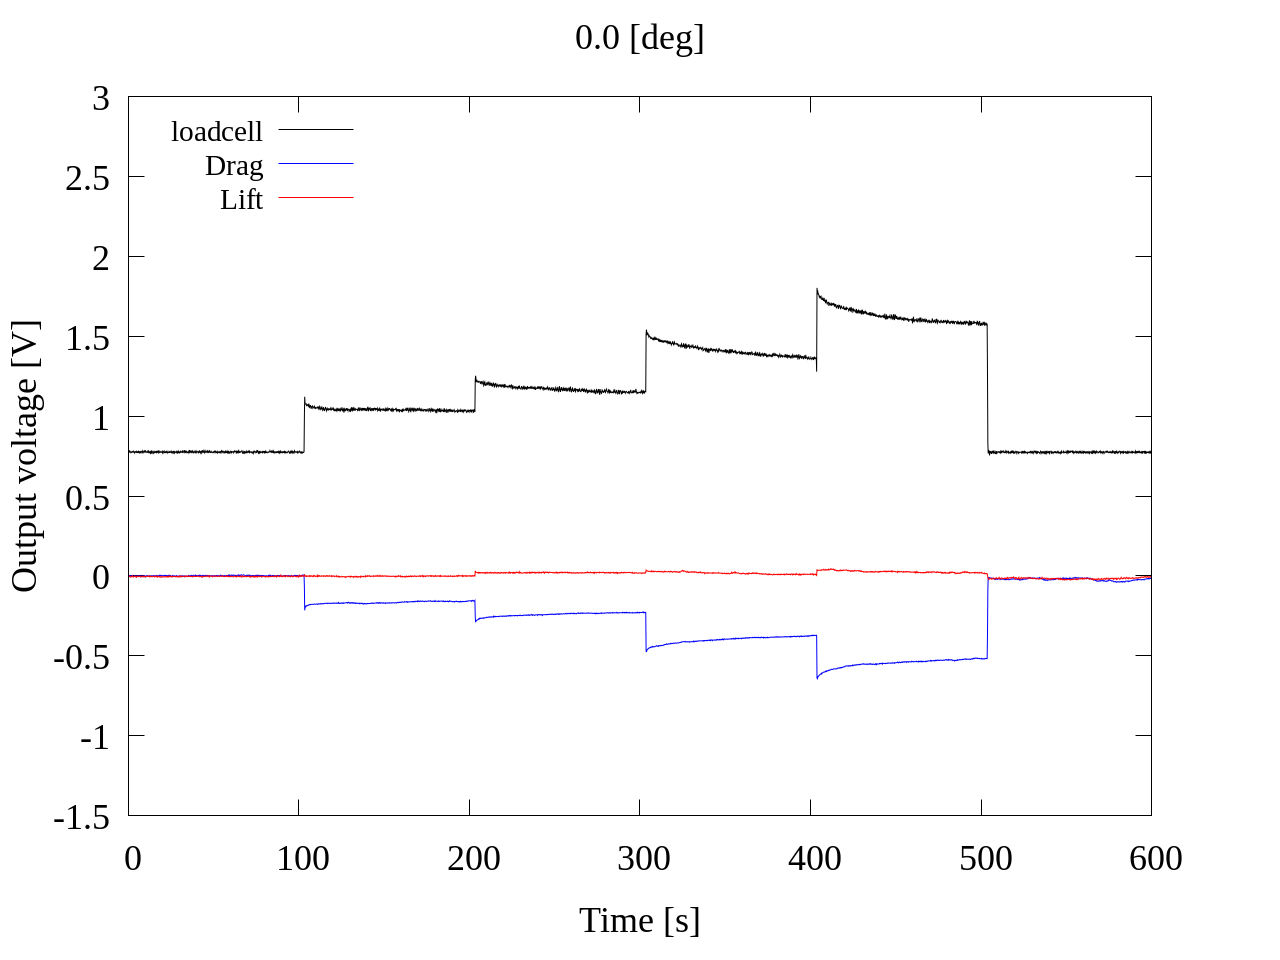
\includegraphics[width=70mm]{../../02_workspace/result/2-1/plot/01-3_allsensors/01_allsensors_0.png}
            \caption{Output voltage : 0 [deg]}
            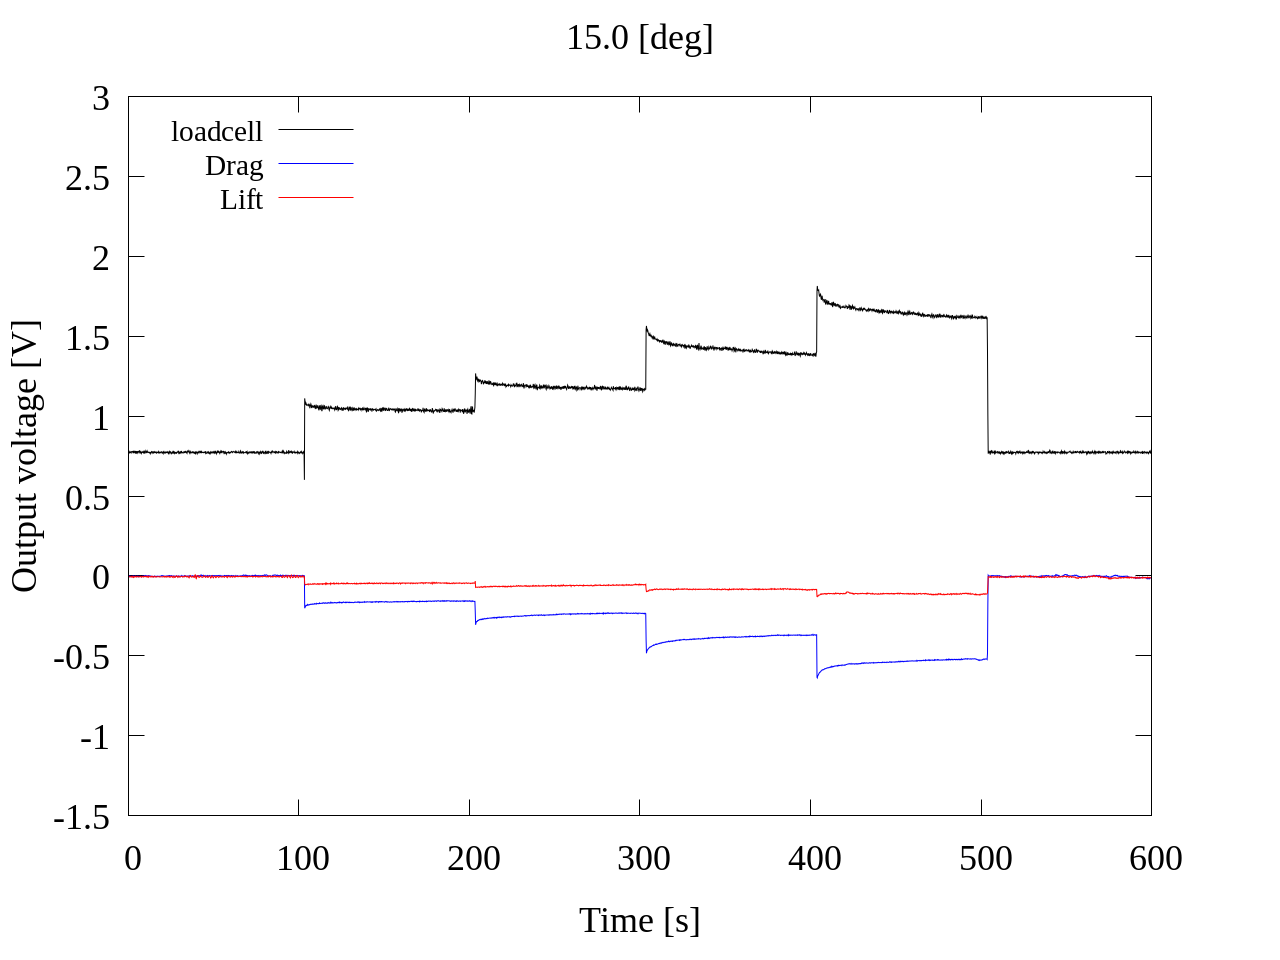
\includegraphics[width=70mm]{../../02_workspace/result/2-1/plot/01-3_allsensors/01_allsensors_150.png}
            \caption{Output voltage : 15 [deg]}
            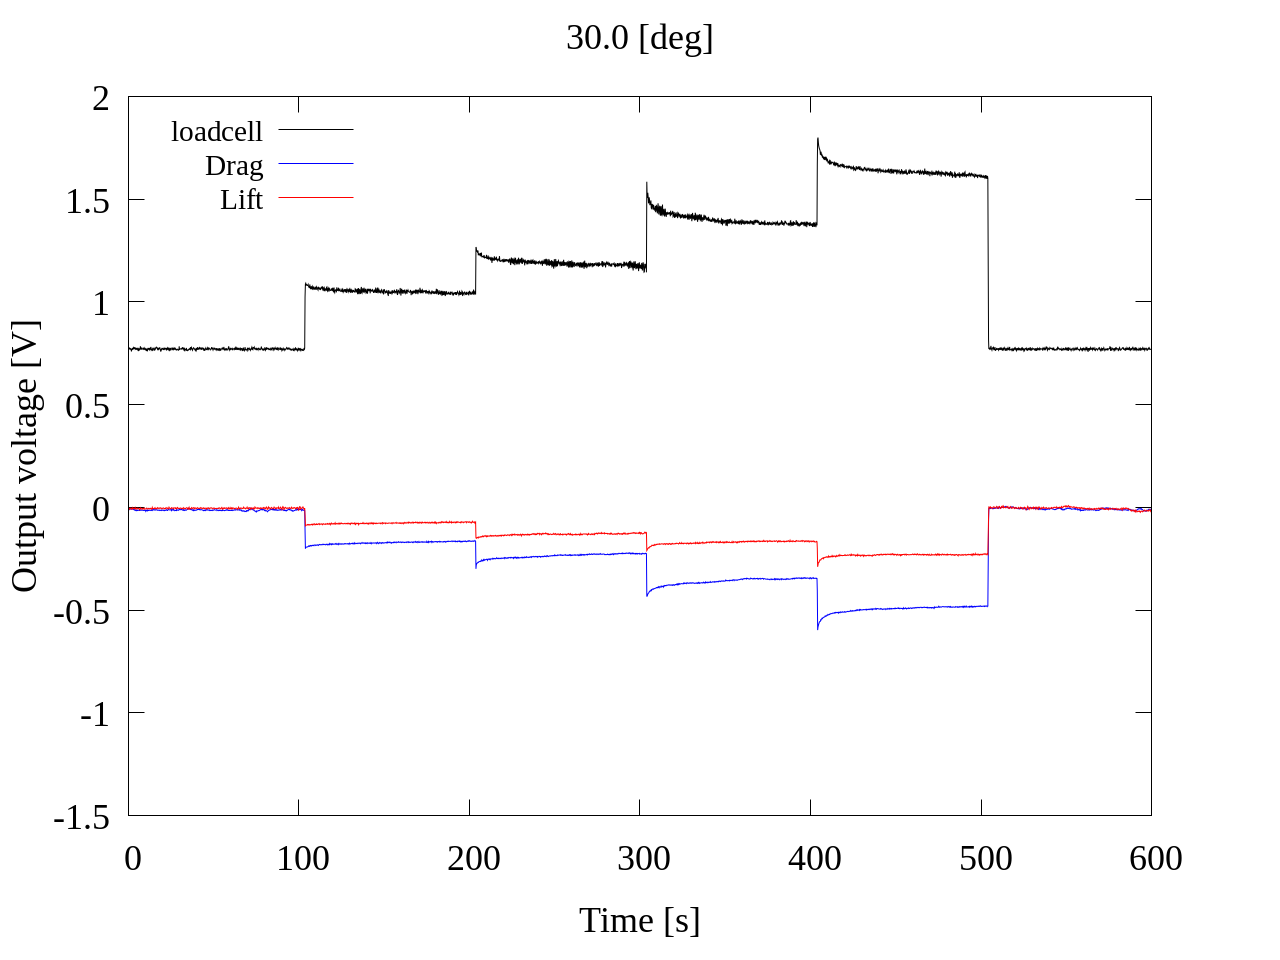
\includegraphics[width=70mm]{../../02_workspace/result/2-1/plot/01-3_allsensors/01_allsensors_300.png}
            \caption{Output voltage : 30 [deg]}
            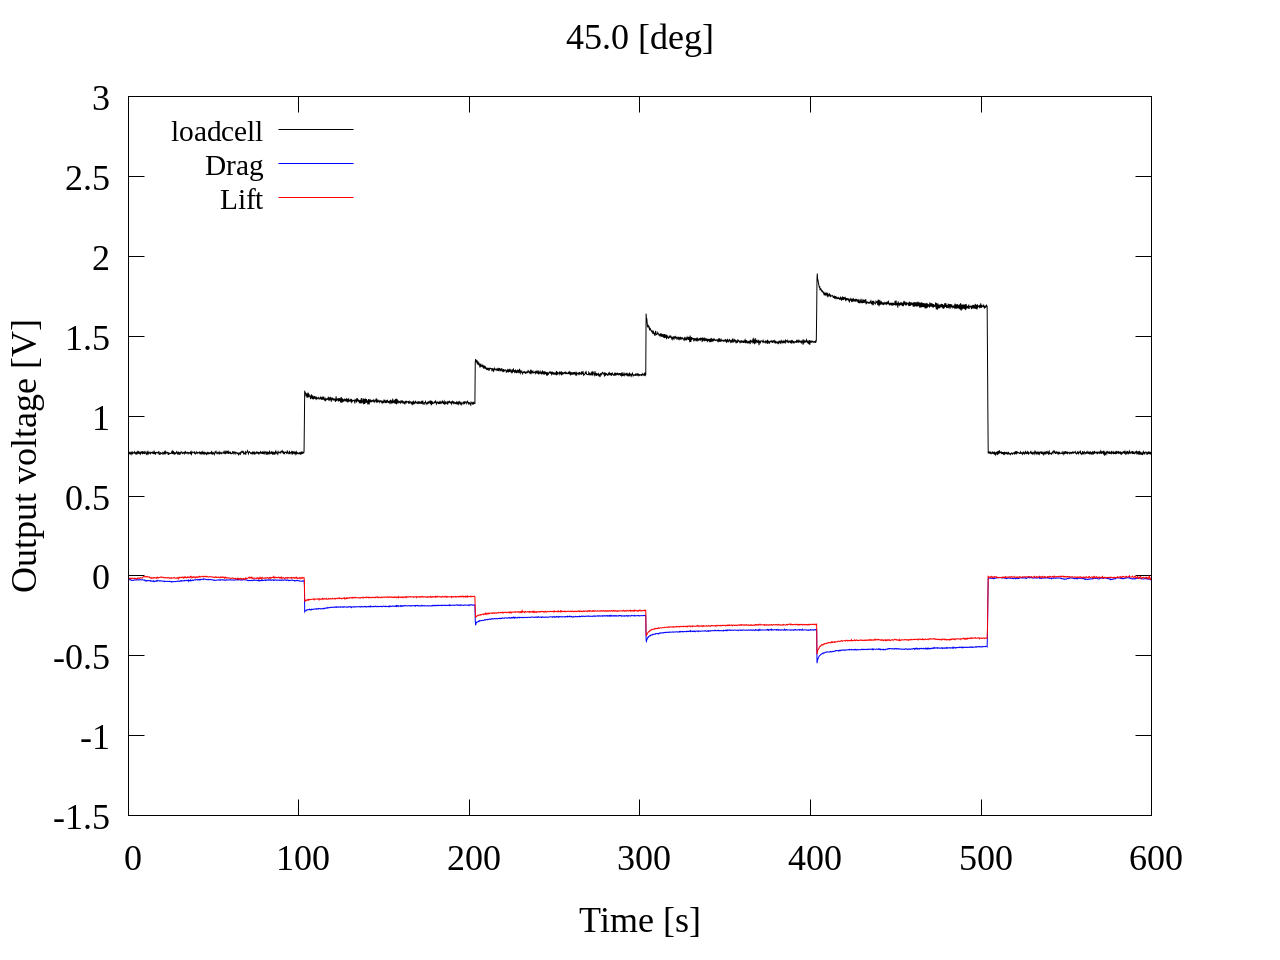
\includegraphics[width=70mm]{../../02_workspace/result/2-1/plot/01-3_allsensors/01_allsensors_450.png}
            \caption{Output voltage : 45 [deg]}
            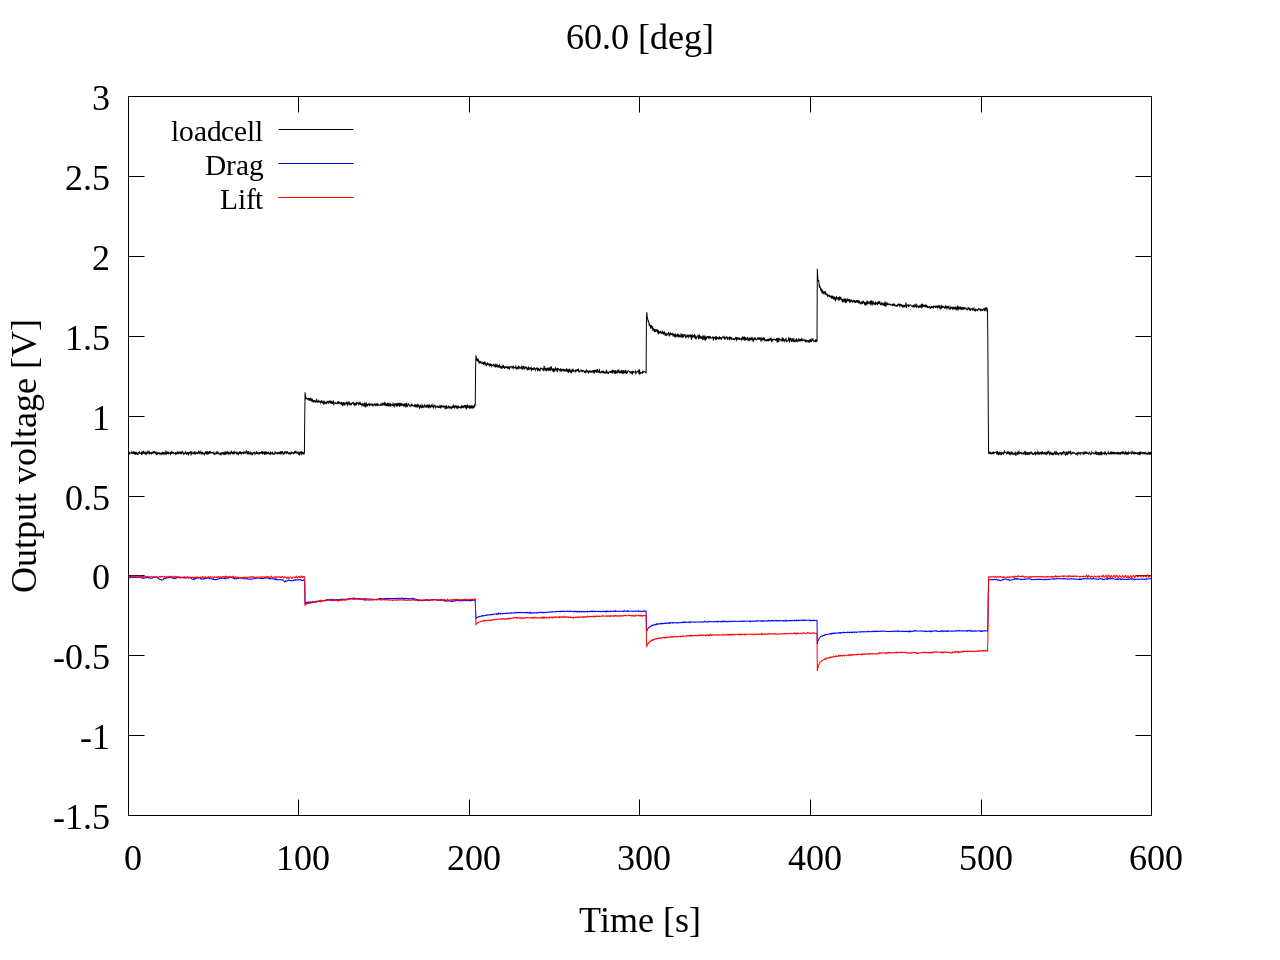
\includegraphics[width=70mm]{../../02_workspace/result/2-1/plot/01-3_allsensors/01_allsensors_600.png}
            \caption{Output voltage : 60 [deg]}
            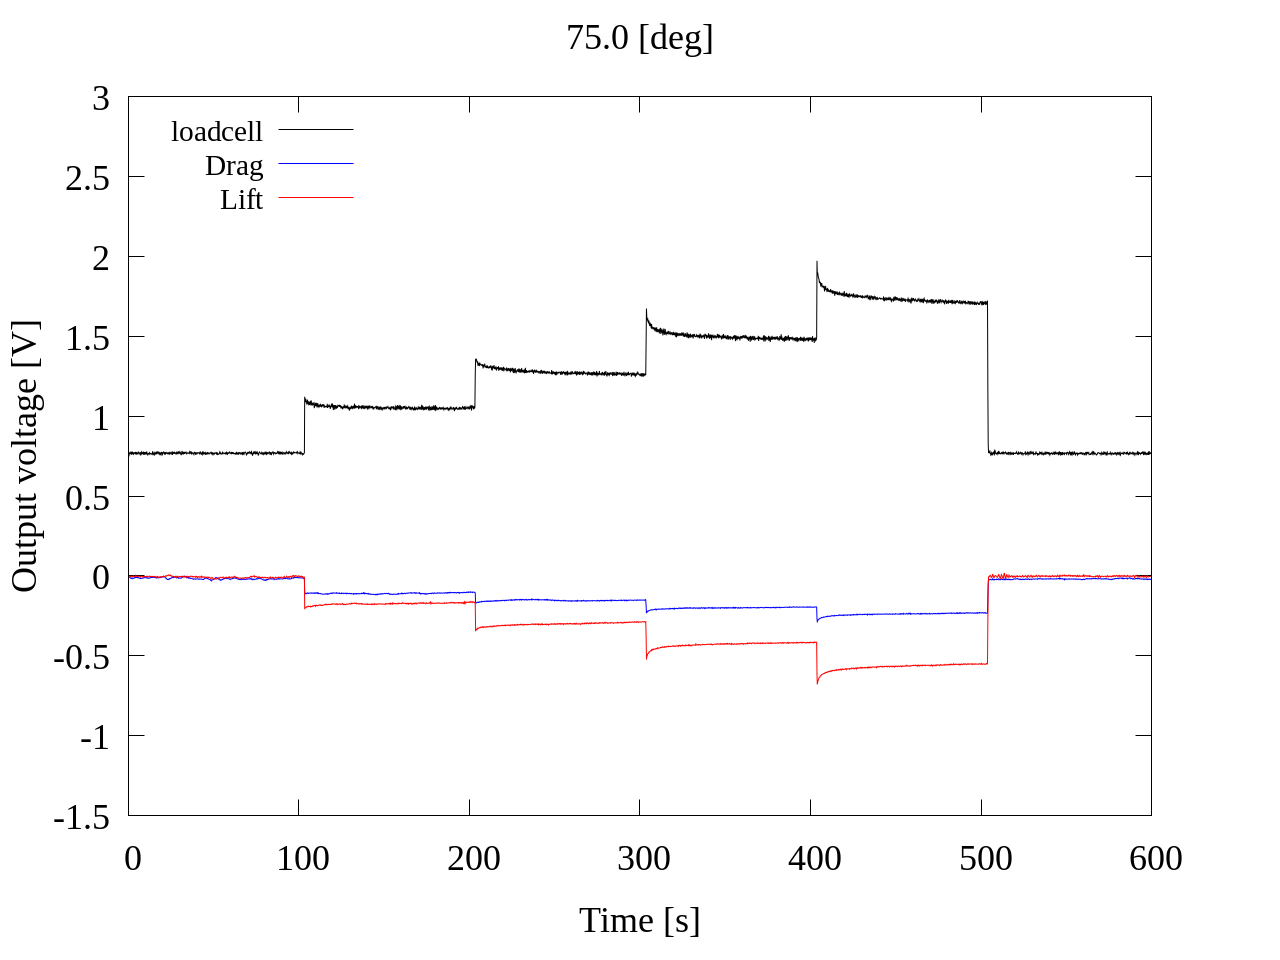
\includegraphics[width=70mm]{../../02_workspace/result/2-1/plot/01-3_allsensors/01_allsensors_750.png}
            \caption{Output voltage : 75 [deg]}
            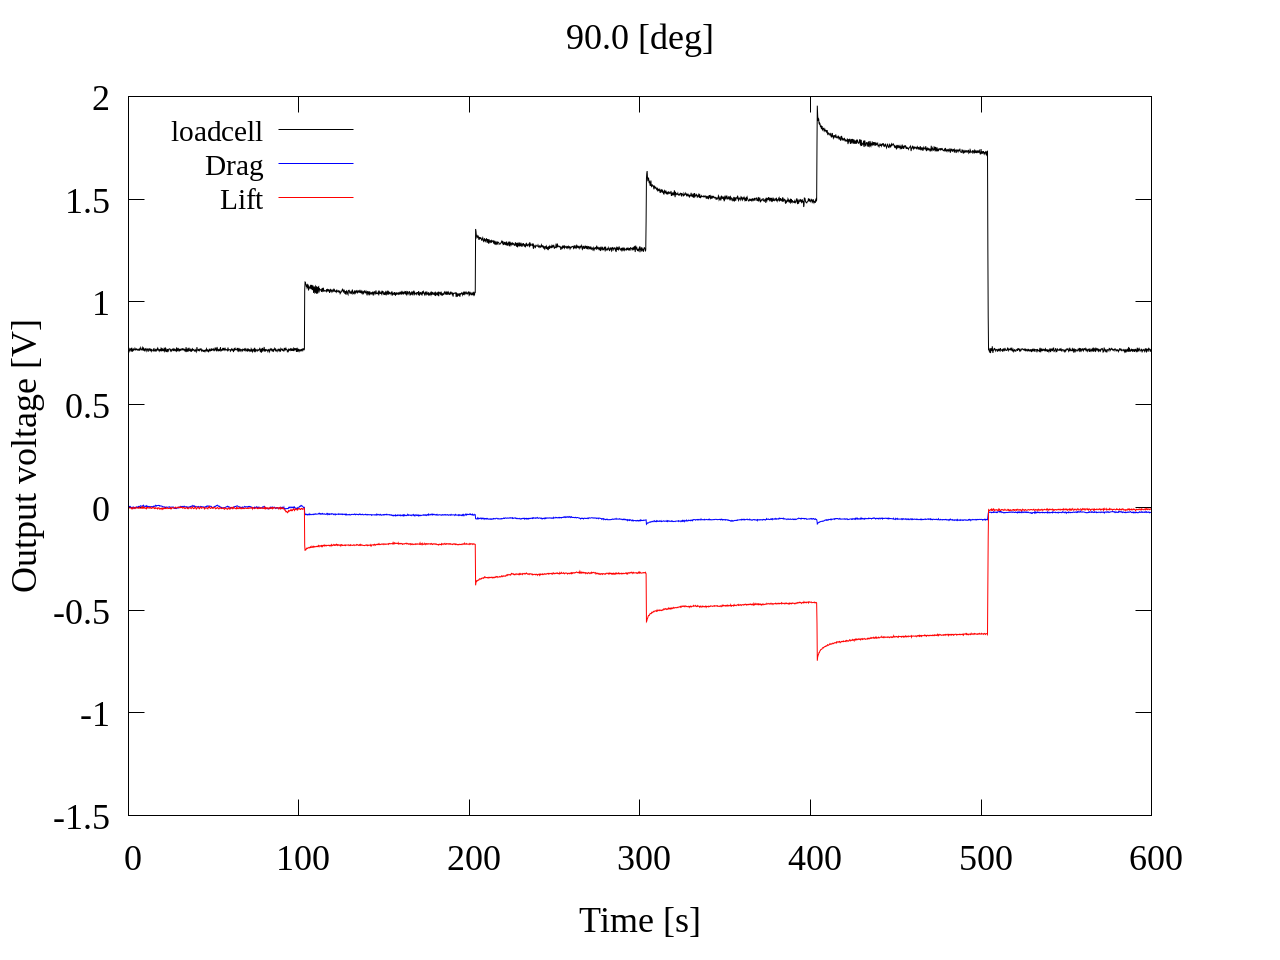
\includegraphics[width=70mm]{../../02_workspace/result/2-1/plot/01-3_allsensors/01_allsensors_900.png}
            \caption{Output voltage : 90 [deg]}
            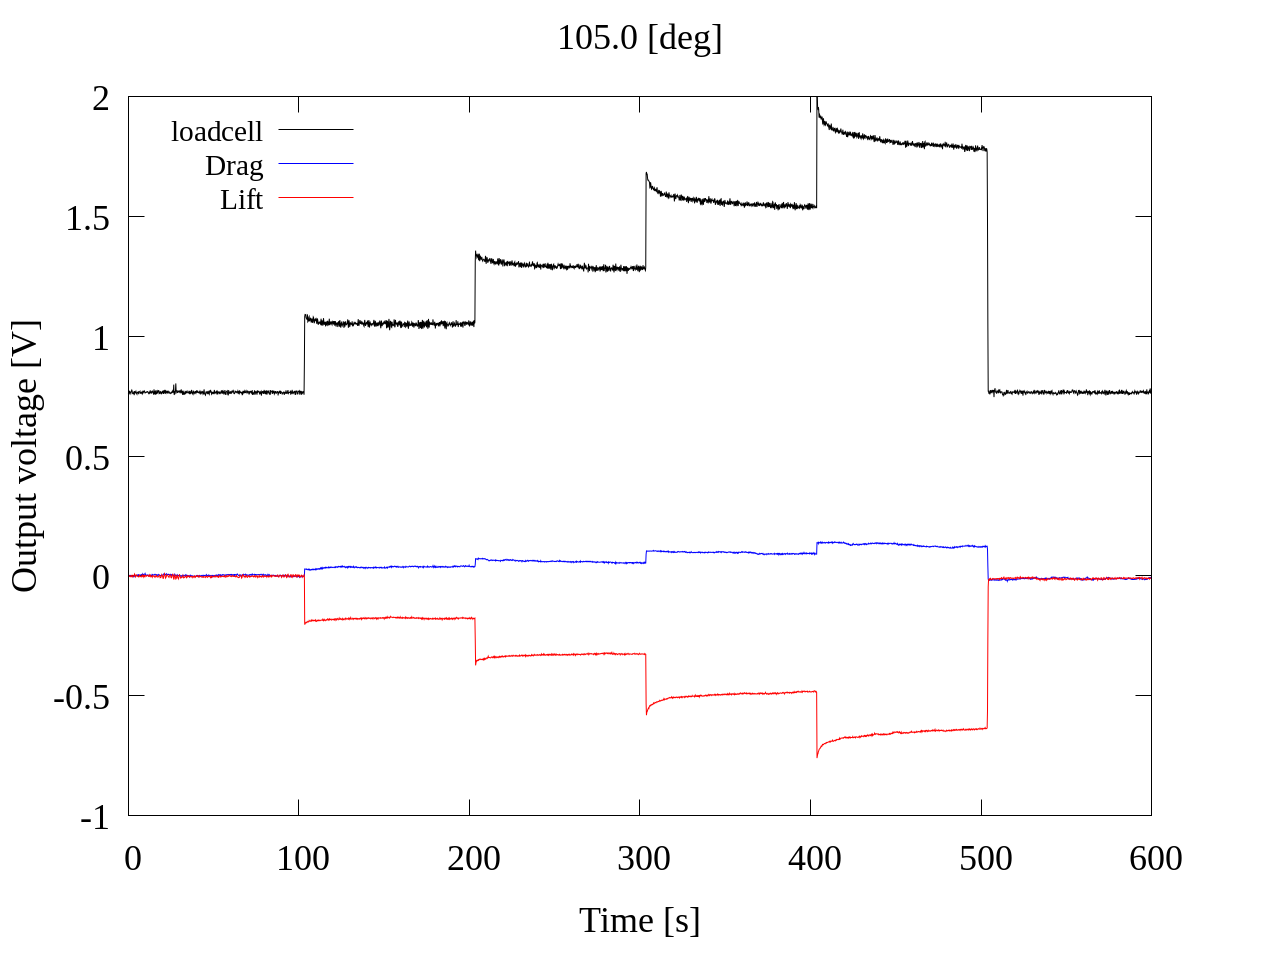
\includegraphics[width=70mm]{../../02_workspace/result/2-1/plot/01-3_allsensors/01_allsensors_1050.png}
            \caption{Output voltage : 105 [deg]}
            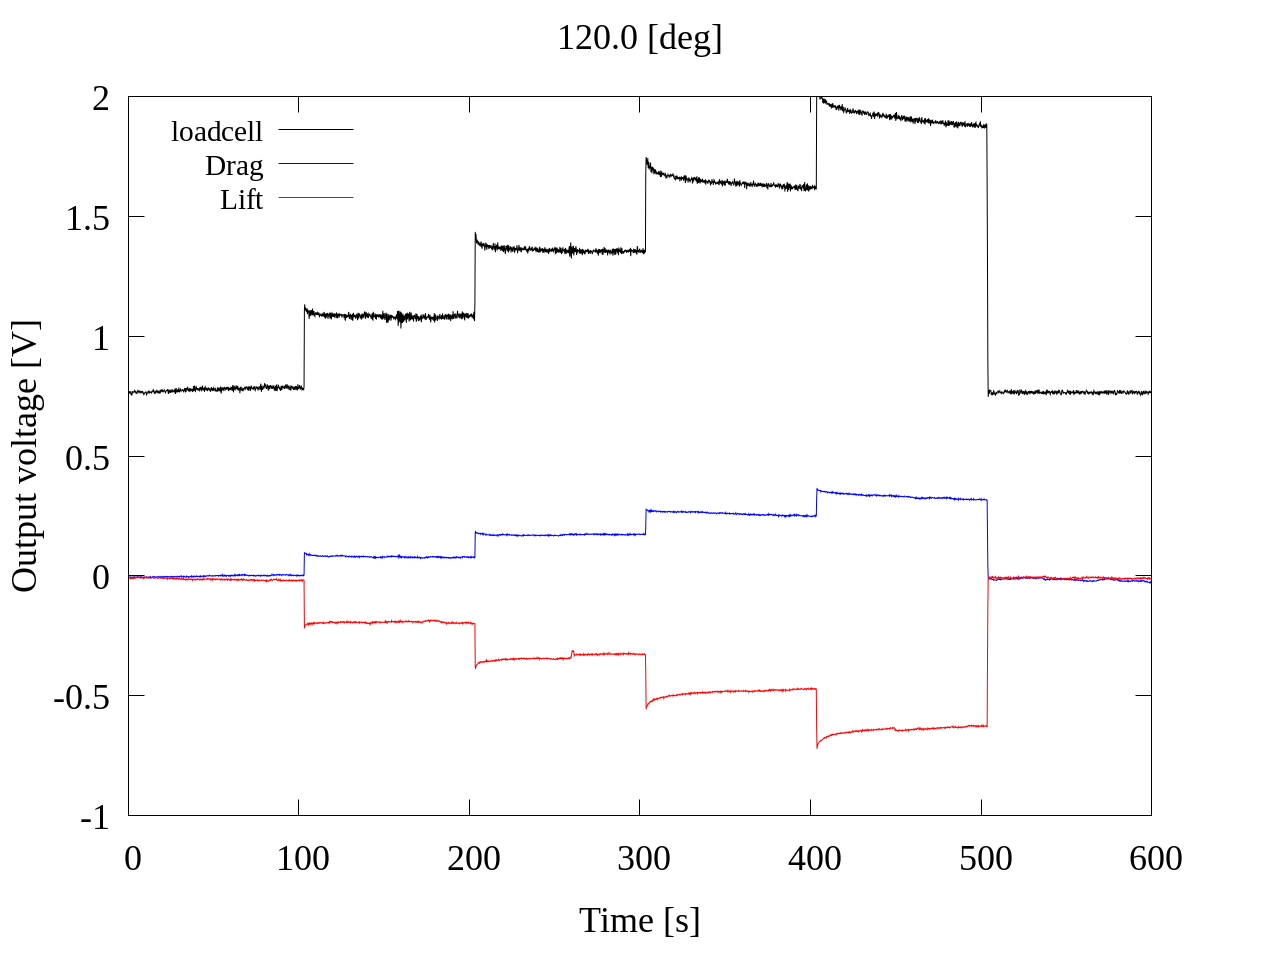
\includegraphics[width=70mm]{../../02_workspace/result/2-1/plot/01-3_allsensors/01_allsensors_1200.png}
            \caption{Output voltage : 120 [deg]}
            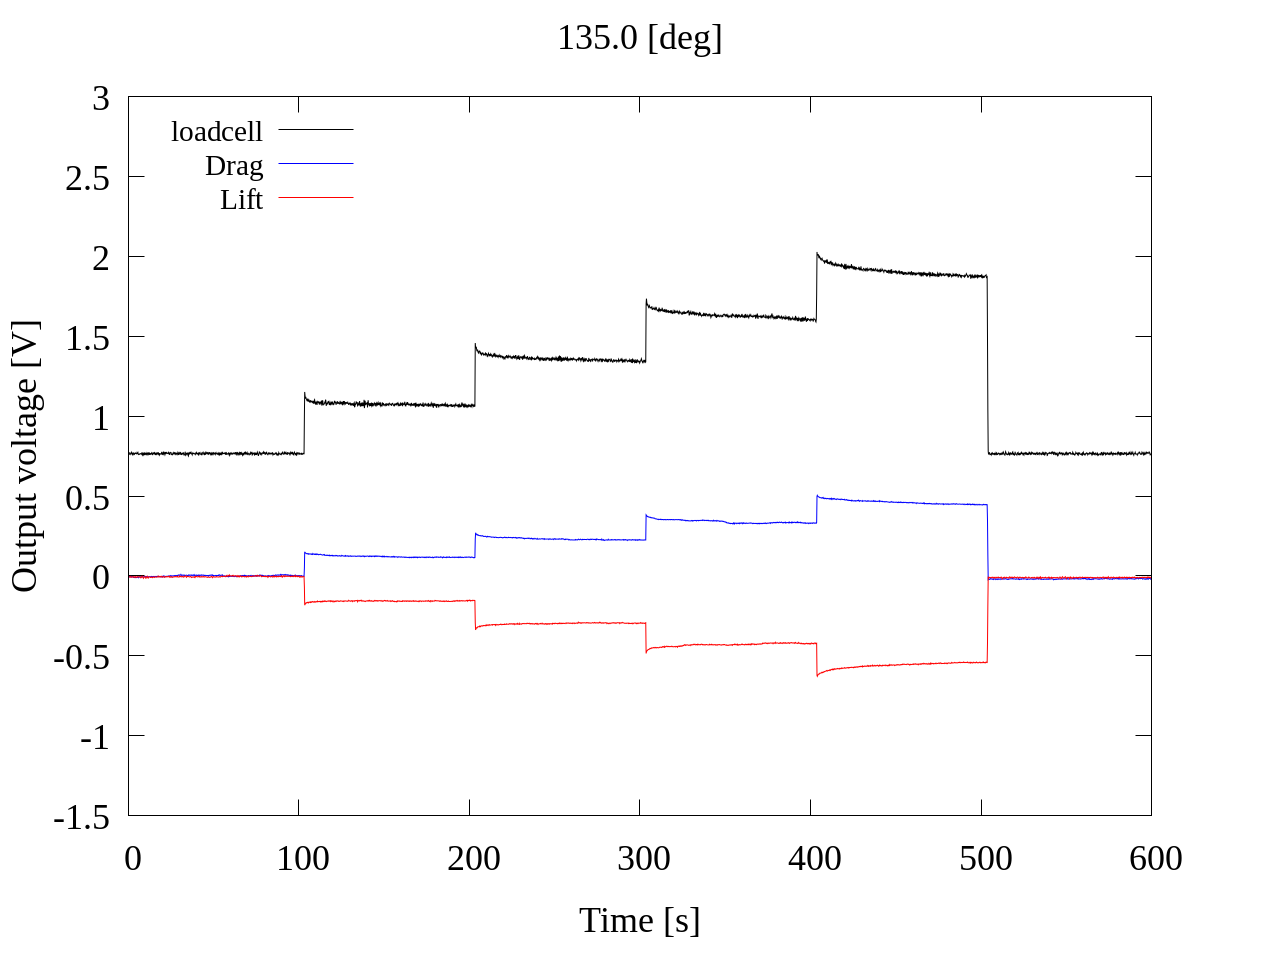
\includegraphics[width=70mm]{../../02_workspace/result/2-1/plot/01-3_allsensors/01_allsensors_1350.png}
            \caption{Output voltage : 135 [deg]}
            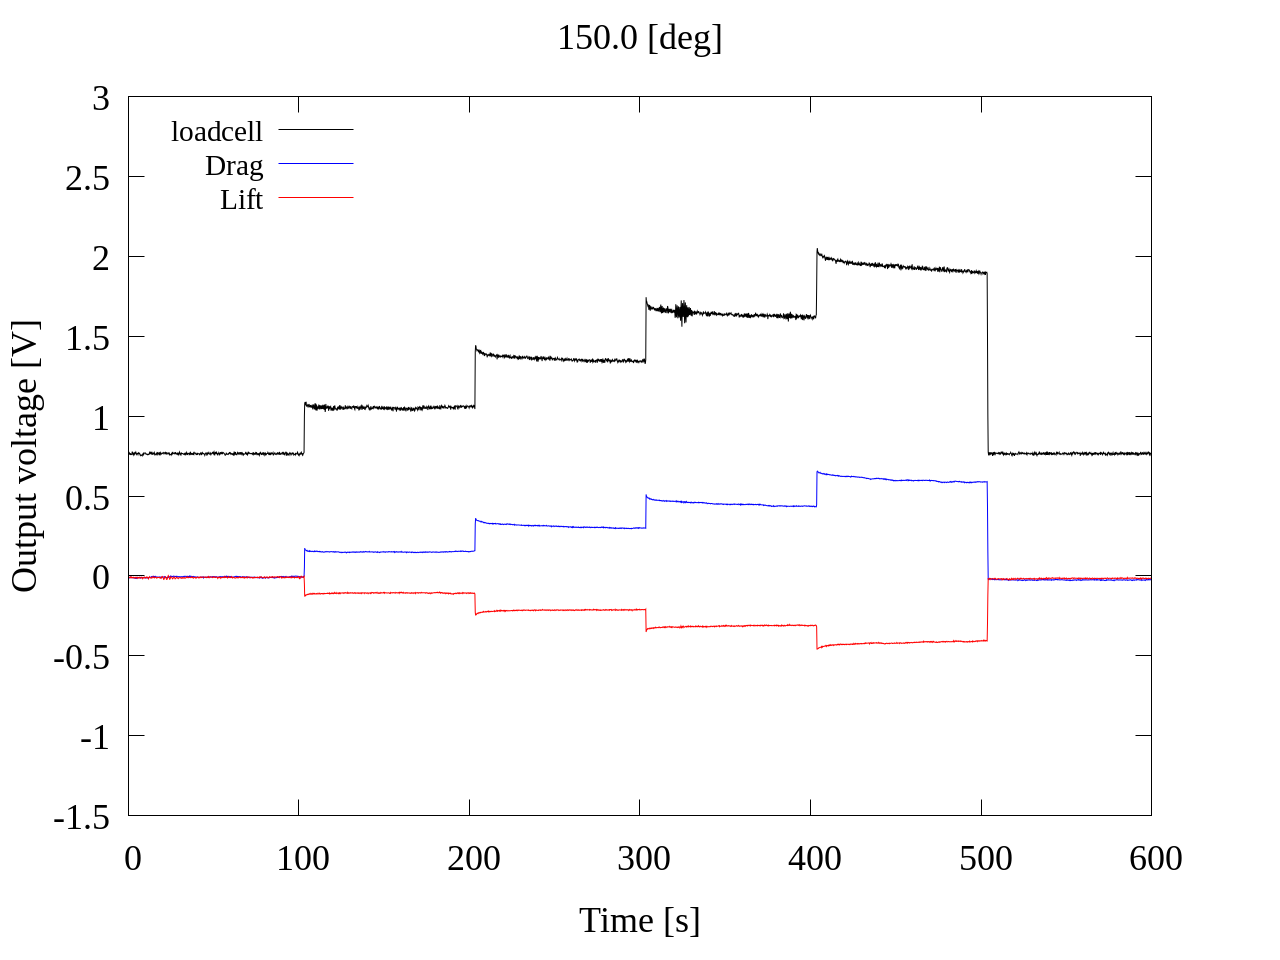
\includegraphics[width=70mm]{../../02_workspace/result/2-1/plot/01-3_allsensors/01_allsensors_1500.png}
            \caption{Output voltage : 150 [deg]}
            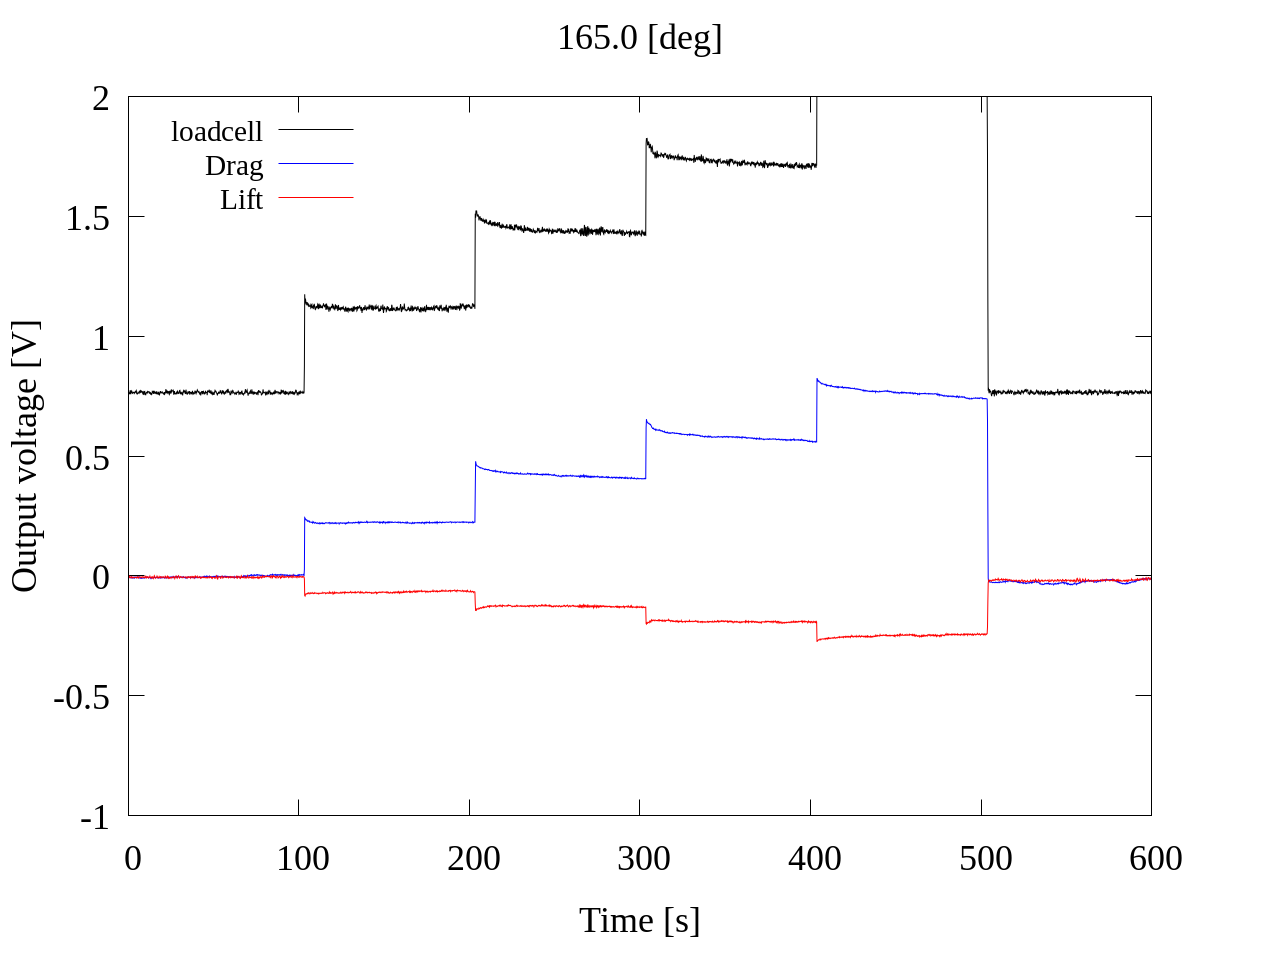
\includegraphics[width=70mm]{../../02_workspace/result/2-1/plot/01-3_allsensors/01_allsensors_1650.png}
            \caption{Output voltage : 165 [deg]}
            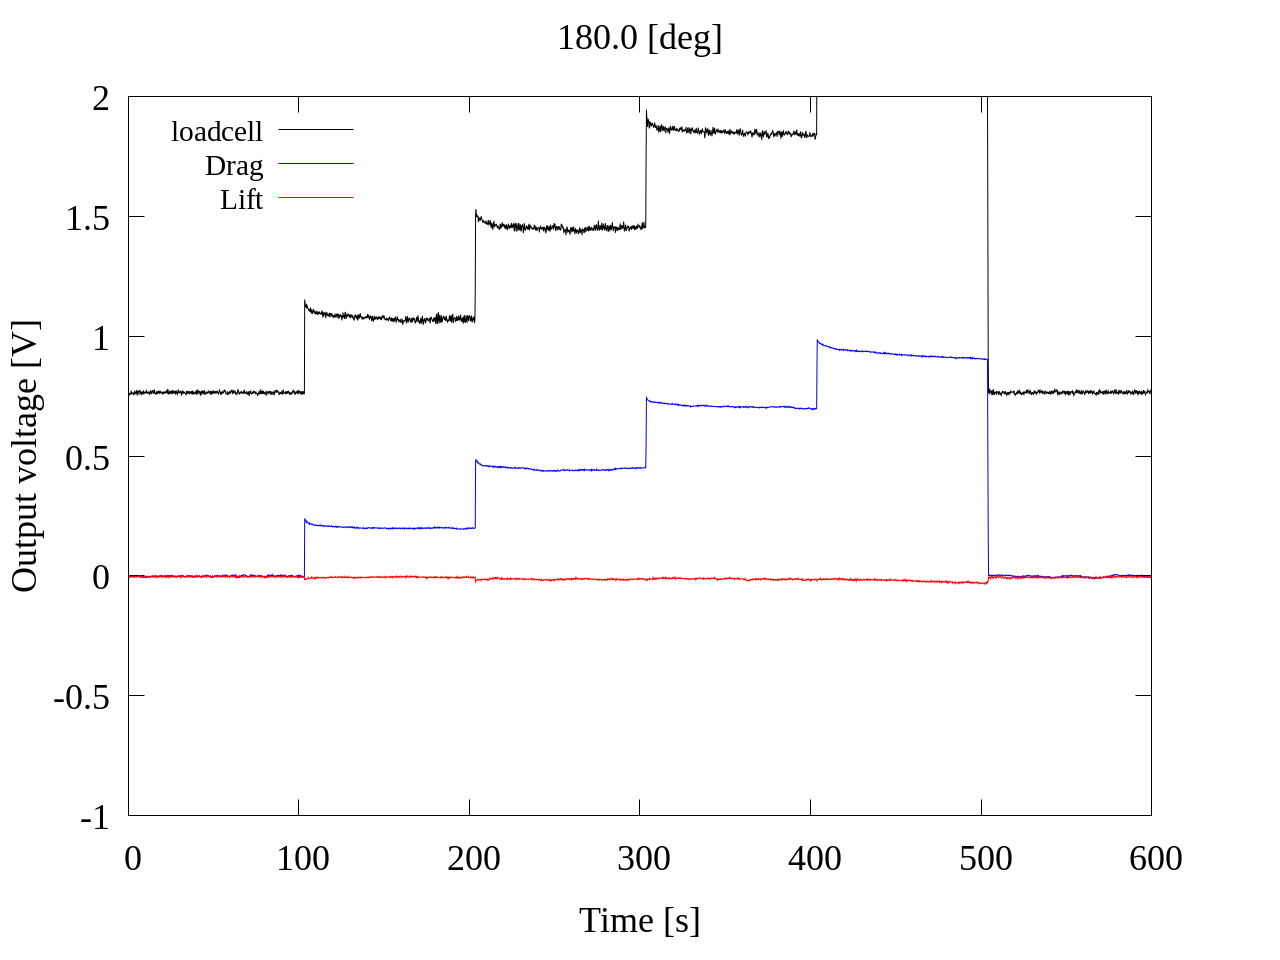
\includegraphics[width=70mm]{../../02_workspace/result/2-1/plot/01-3_allsensors/01_allsensors_1800.png}
            \caption{Output voltage : 180 [deg]}
            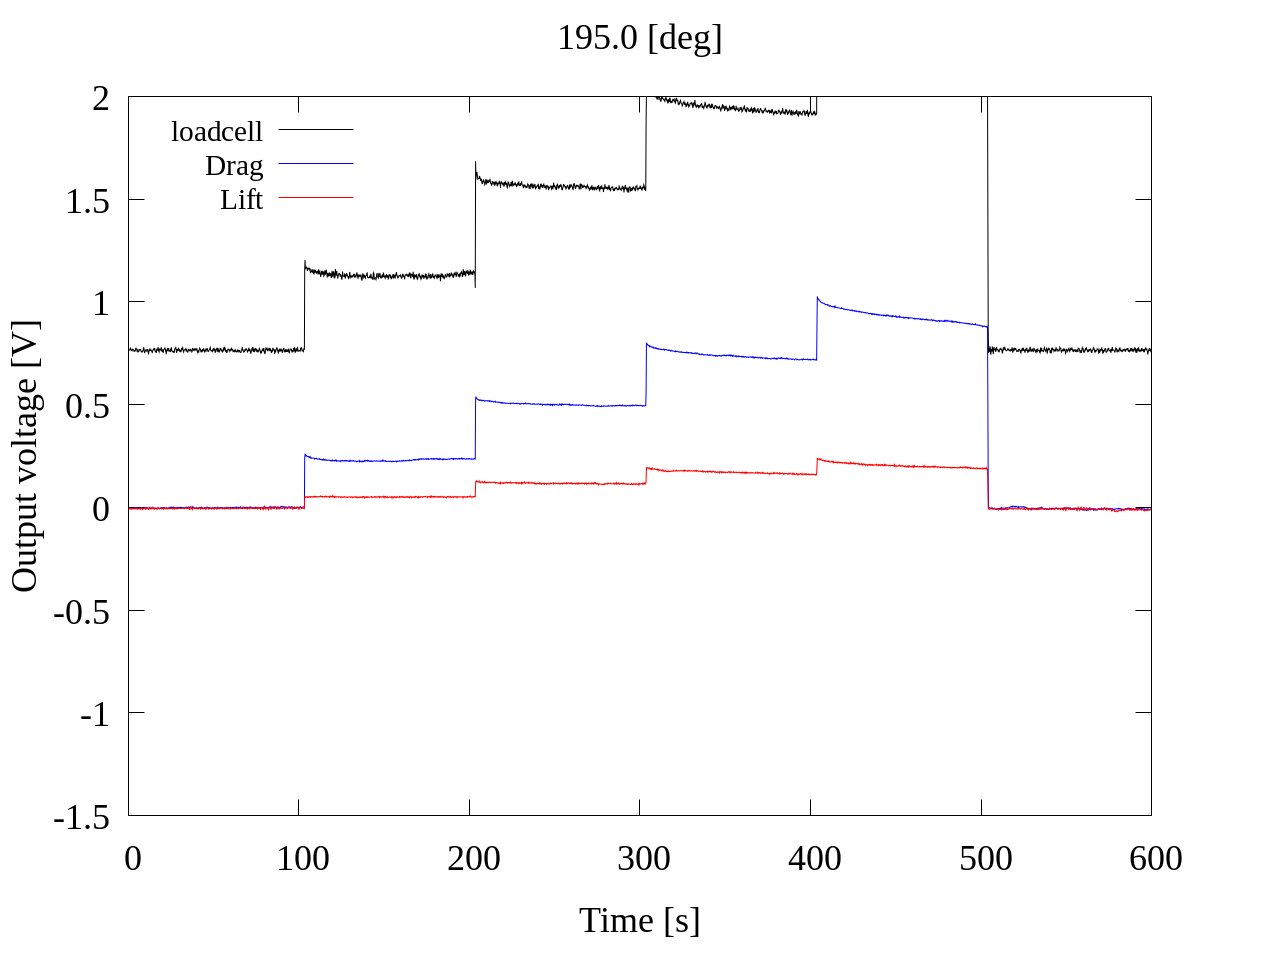
\includegraphics[width=70mm]{../../02_workspace/result/2-1/plot/01-3_allsensors/01_allsensors_1950.png}
            \caption{Output voltage : 195 [deg]}
            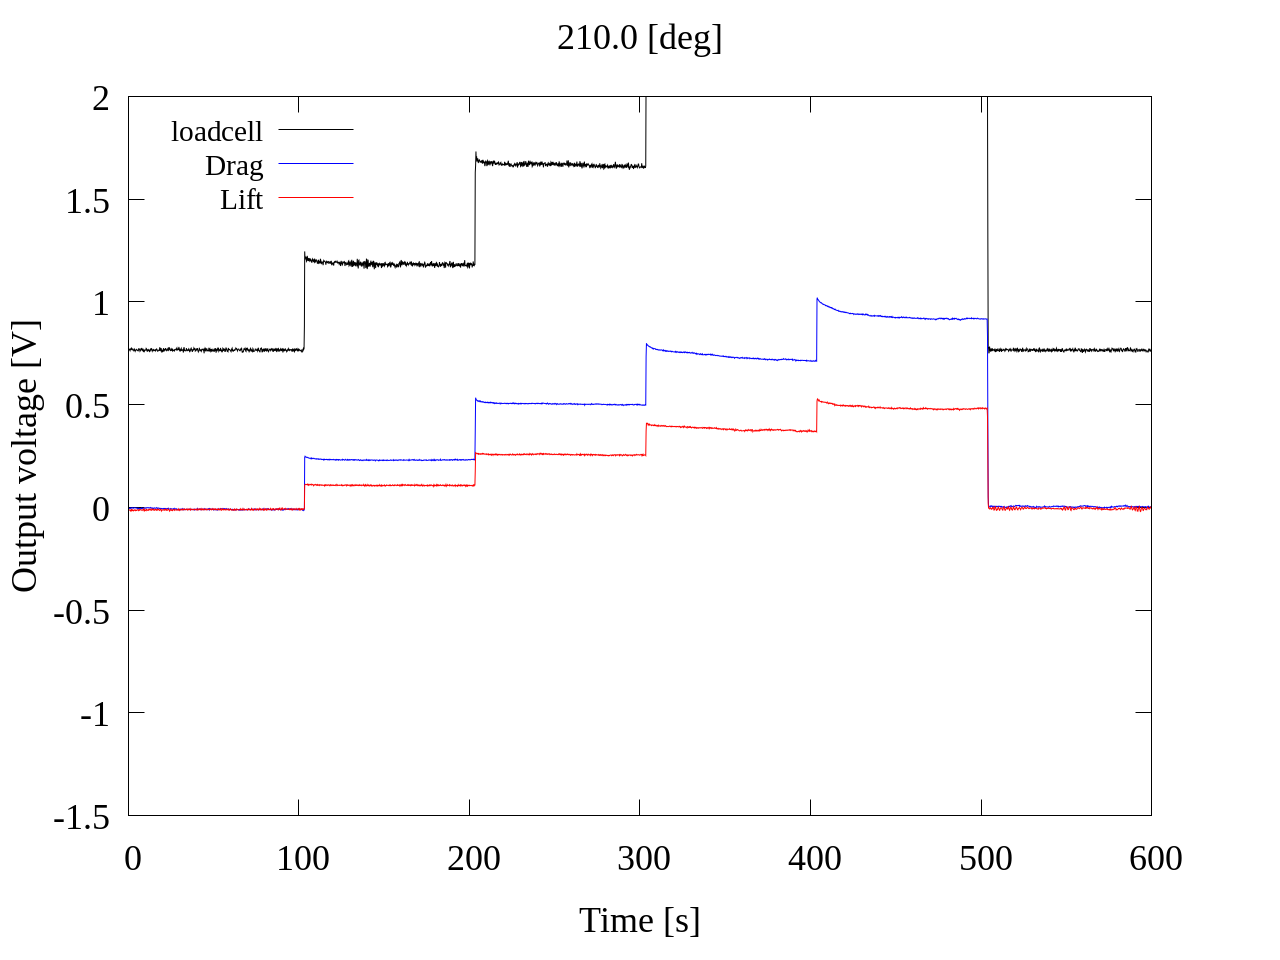
\includegraphics[width=70mm]{../../02_workspace/result/2-1/plot/01-3_allsensors/01_allsensors_2100.png}
            \caption{Output voltage : 210 [deg]}
            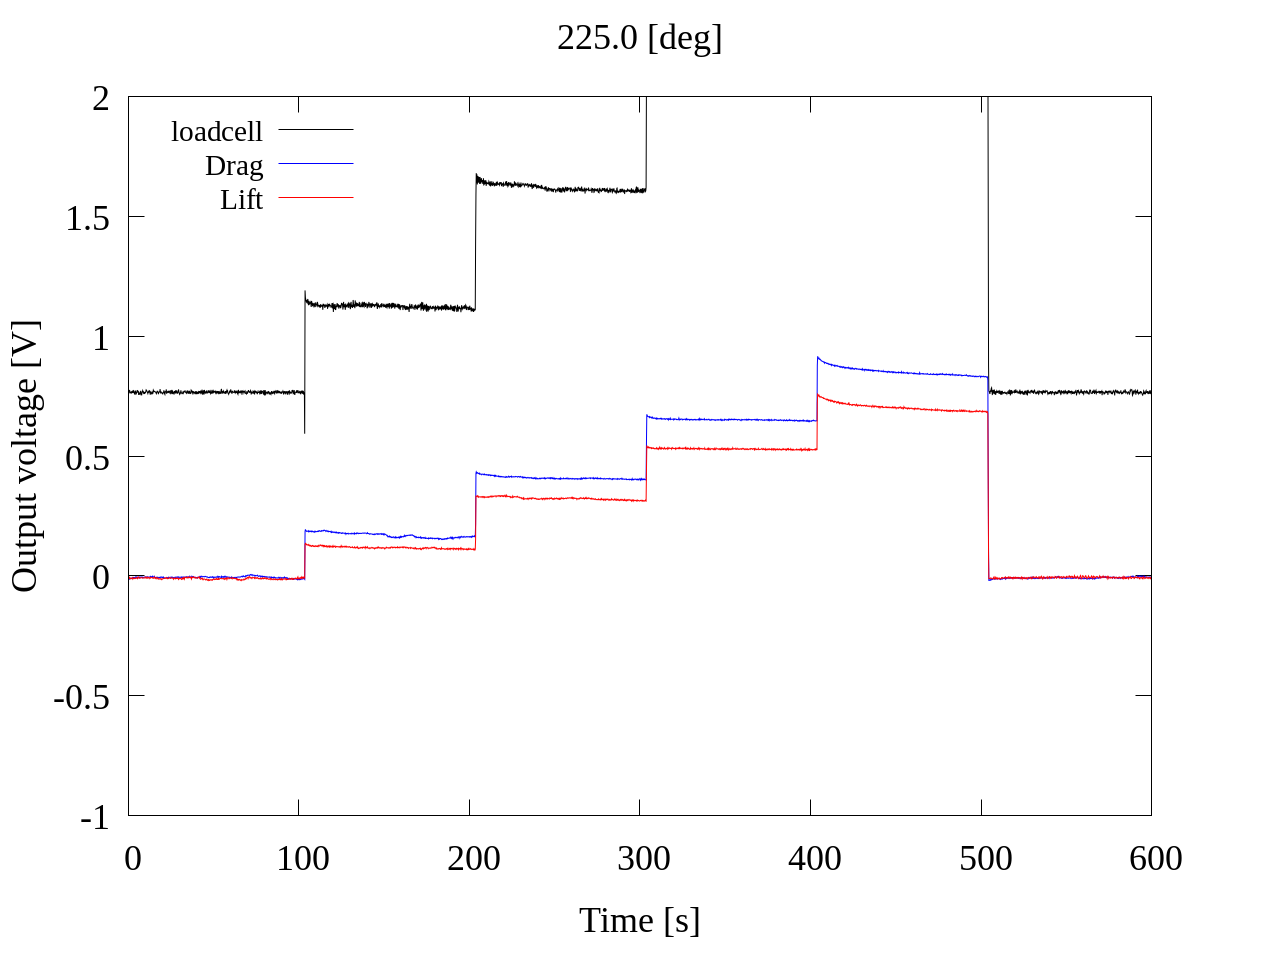
\includegraphics[width=70mm]{../../02_workspace/result/2-1/plot/01-3_allsensors/01_allsensors_2250.png}
            \caption{Output voltage : 225 [deg]}
            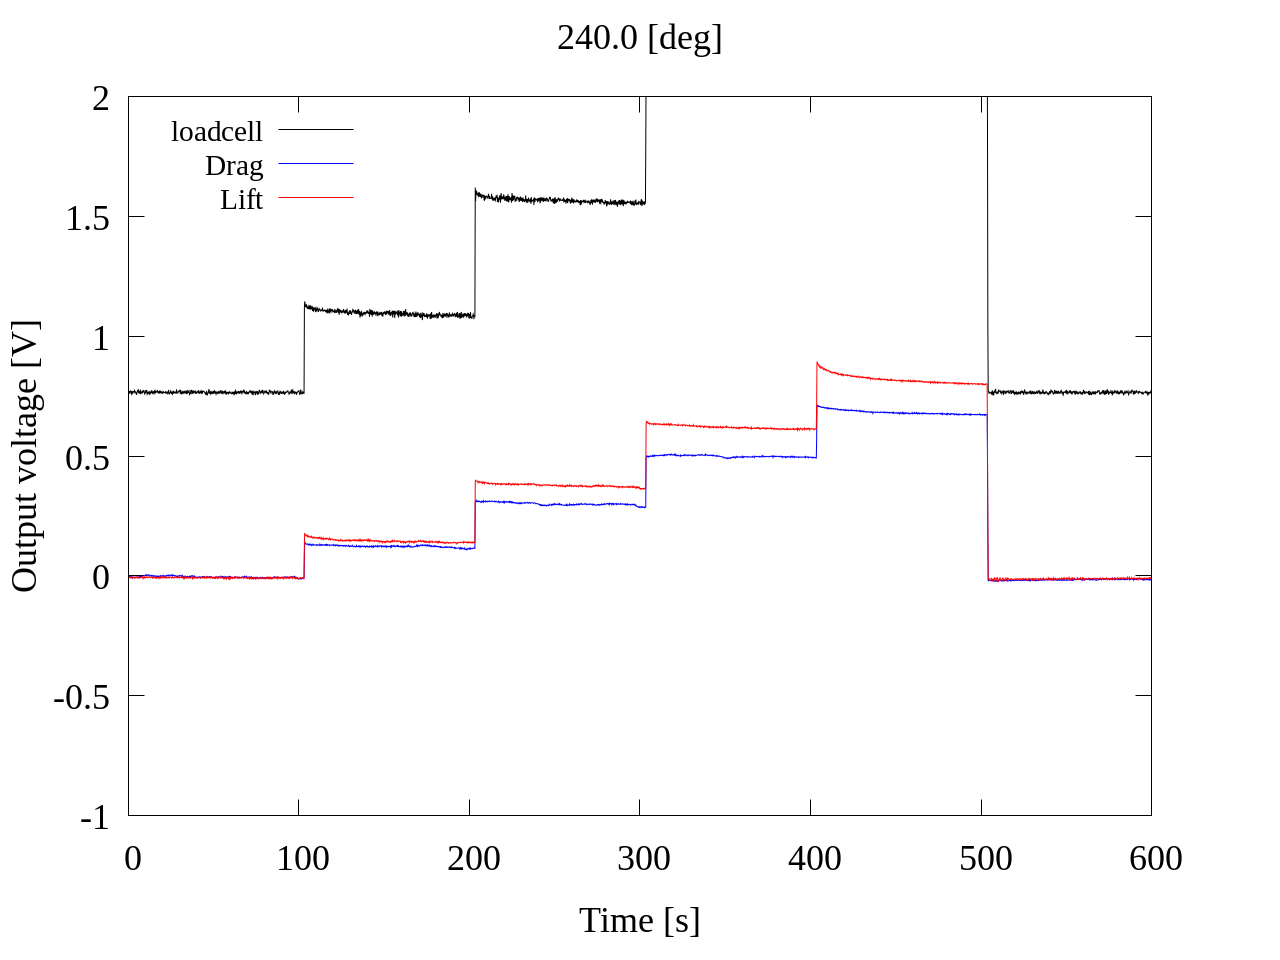
\includegraphics[width=70mm]{../../02_workspace/result/2-1/plot/01-3_allsensors/01_allsensors_2400.png}
            \caption{Output voltage : 240 [deg]}
            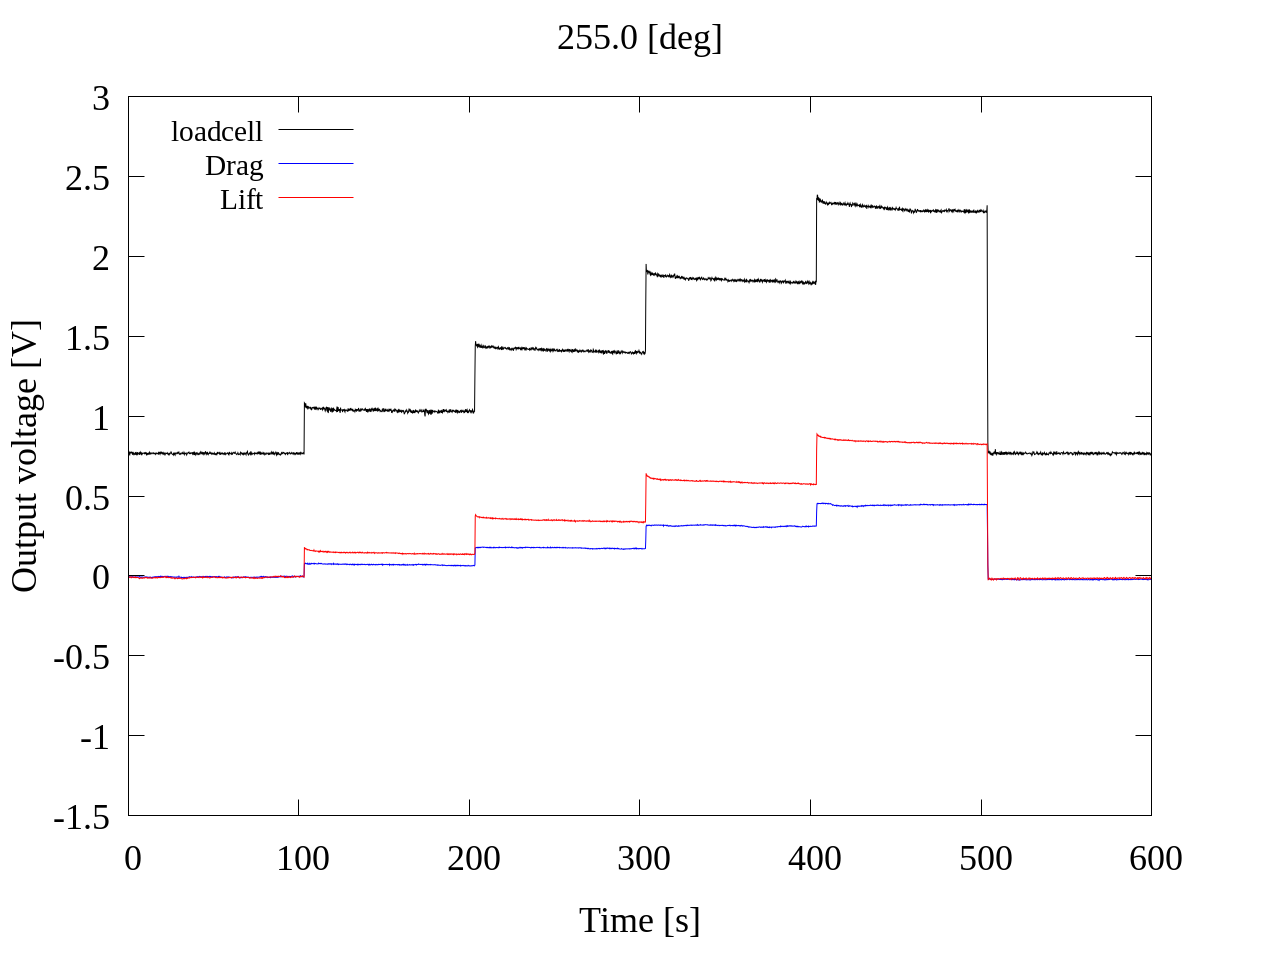
\includegraphics[width=70mm]{../../02_workspace/result/2-1/plot/01-3_allsensors/01_allsensors_2550.png}
            \caption{Output voltage : 255 [deg]}
            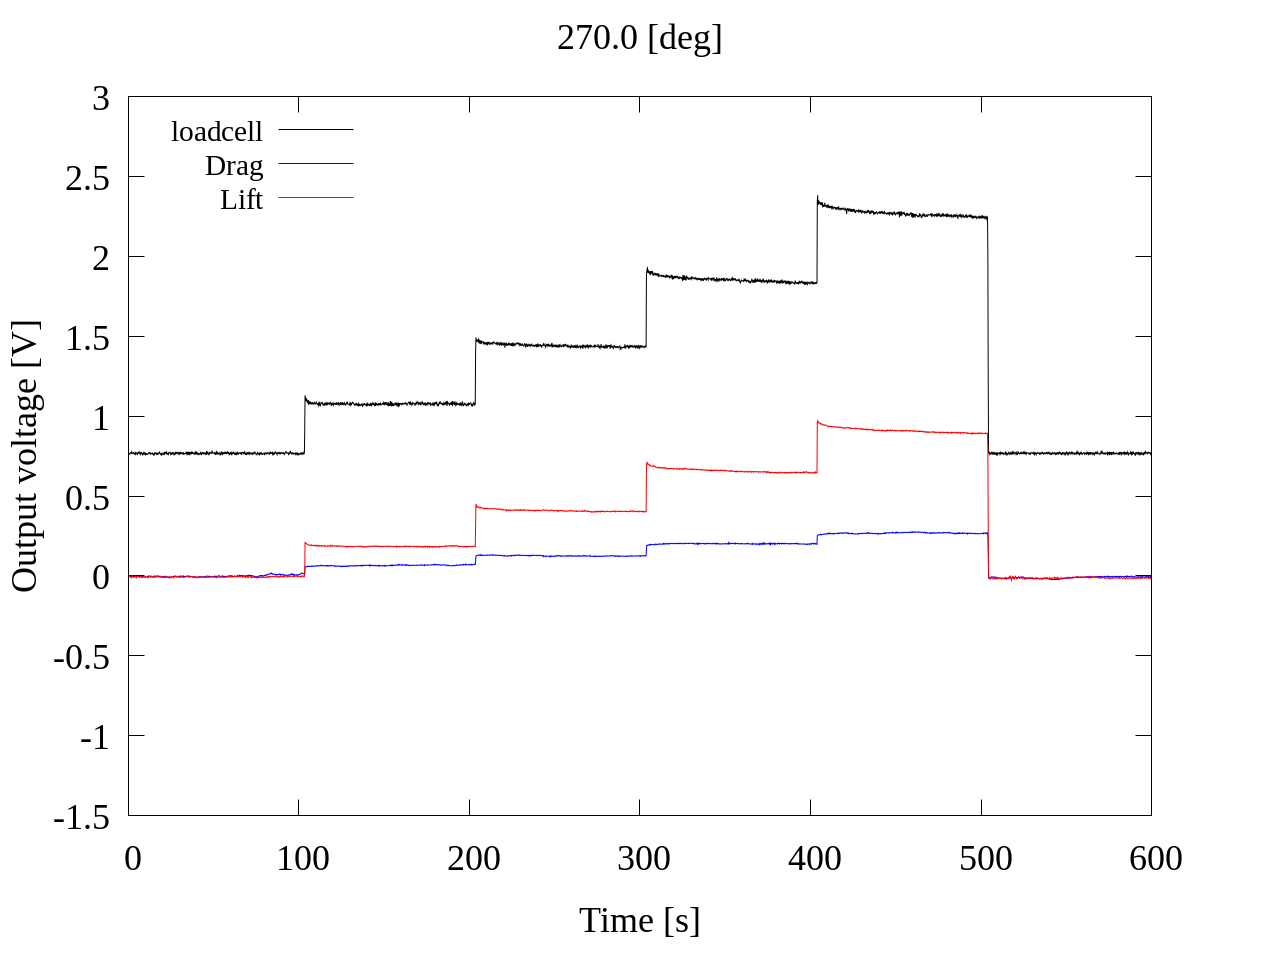
\includegraphics[width=70mm]{../../02_workspace/result/2-1/plot/01-3_allsensors/01_allsensors_2700.png}
            \caption{Output voltage : 270 [deg]}
            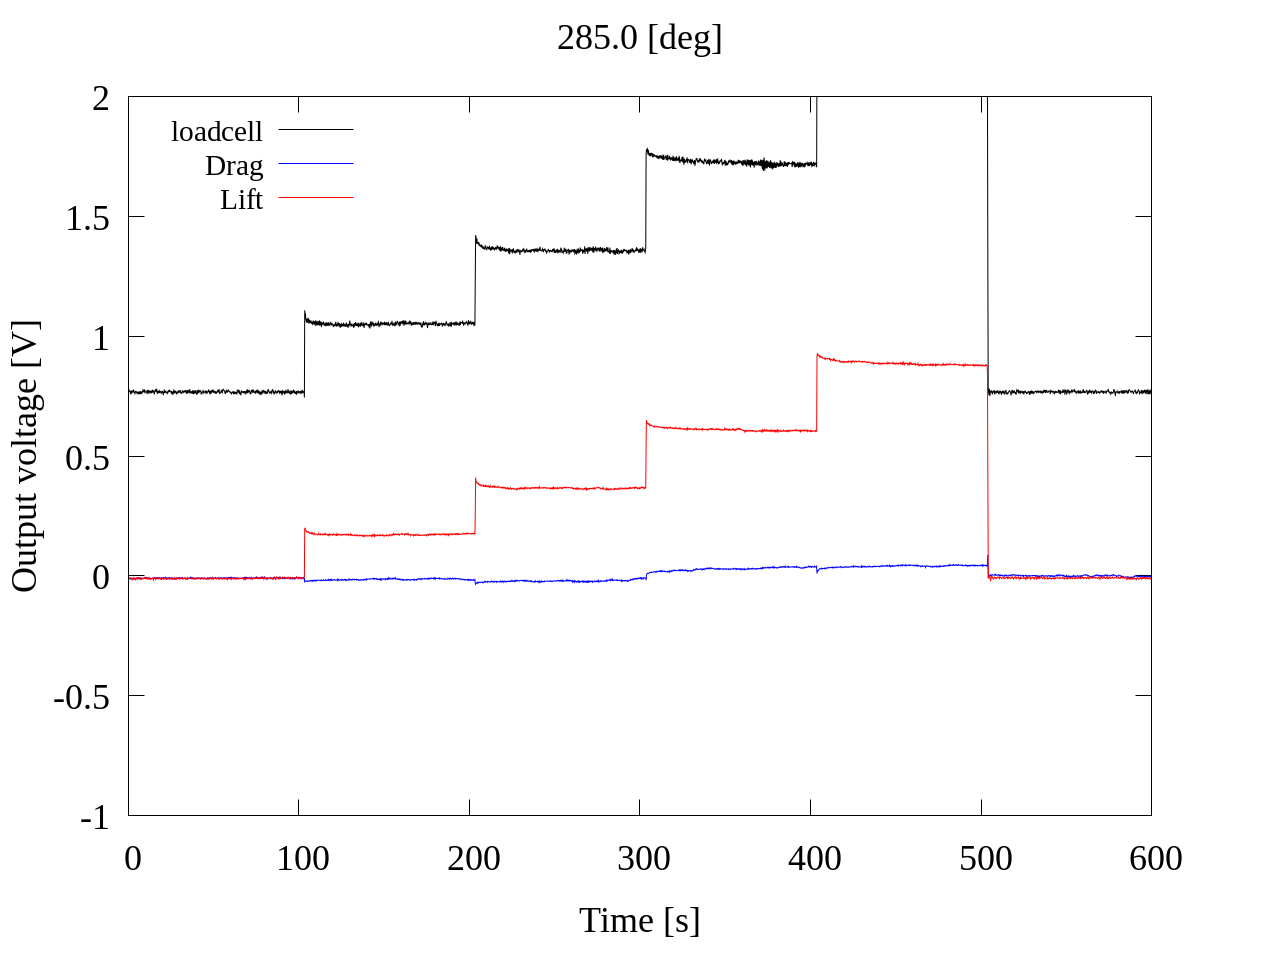
\includegraphics[width=70mm]{../../02_workspace/result/2-1/plot/01-3_allsensors/01_allsensors_2850.png}
            \caption{Output voltage : 285 [deg]}
            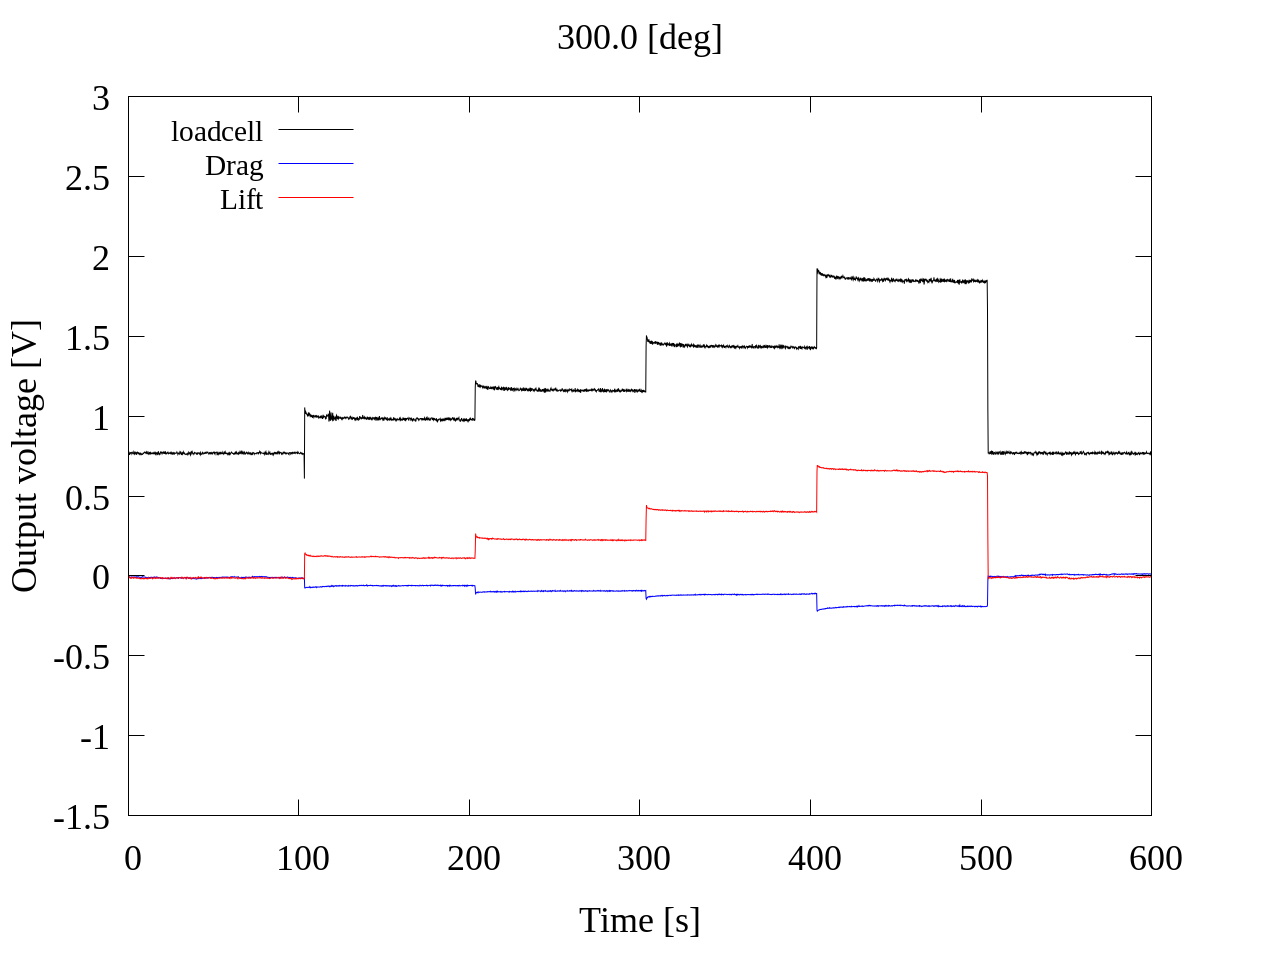
\includegraphics[width=70mm]{../../02_workspace/result/2-1/plot/01-3_allsensors/01_allsensors_3000.png}
            \caption{Output voltage : 300 [deg]}
            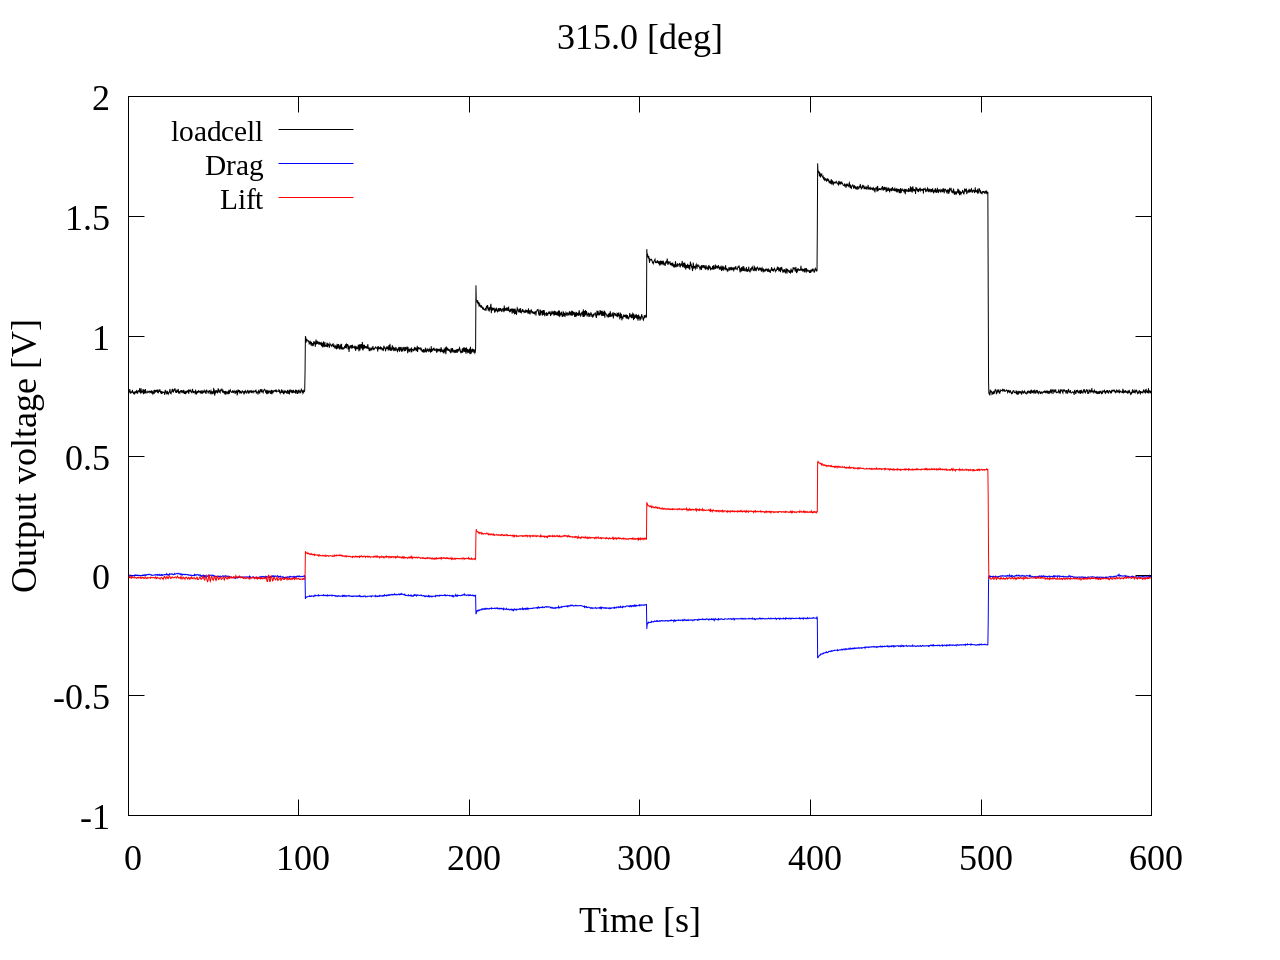
\includegraphics[width=70mm]{../../02_workspace/result/2-1/plot/01-3_allsensors/01_allsensors_3150.png}
            \caption{Output voltage : 315 [deg]}
            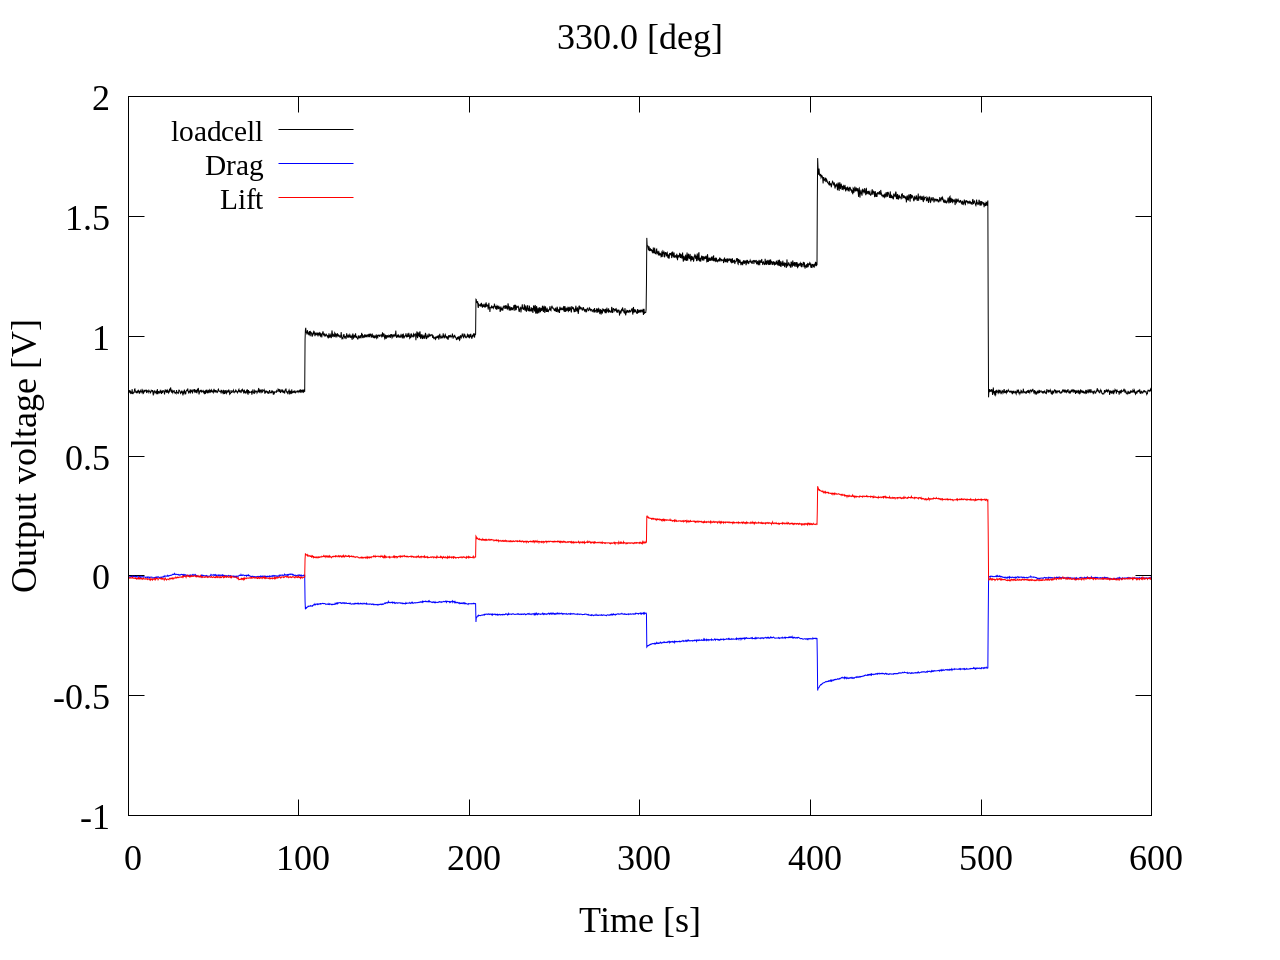
\includegraphics[width=70mm]{../../02_workspace/result/2-1/plot/01-3_allsensors/01_allsensors_3300.png}
            \caption{Output voltage : 330 [deg]}
            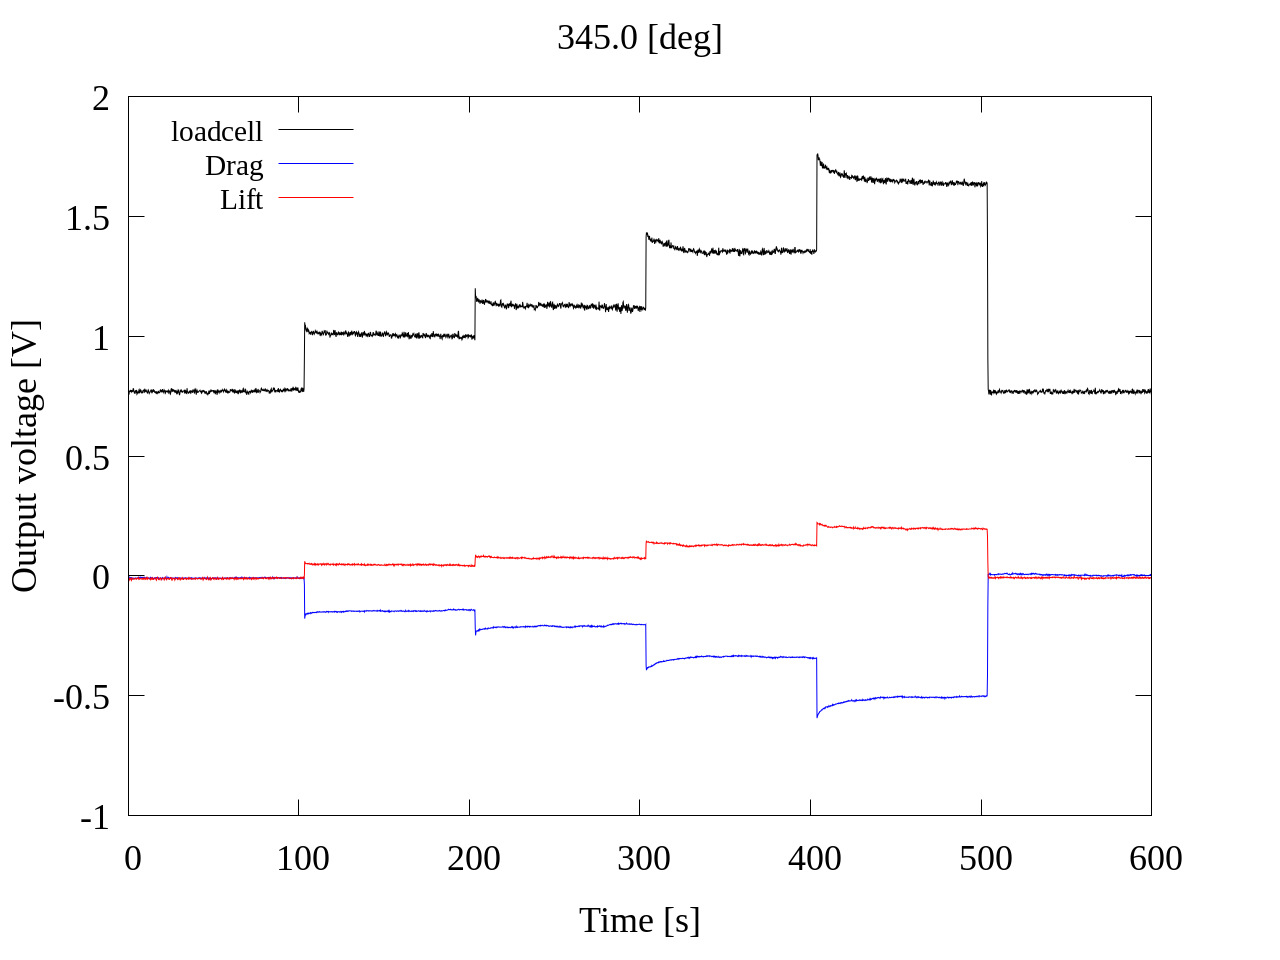
\includegraphics[width=70mm]{../../02_workspace/result/2-1/plot/01-3_allsensors/01_allsensors_3450.png}
            \caption{Output voltage : 345 [deg]}
        \end{center}
    \end{figure_here}
\end{multicols}

以上の結果をみると自動一軸ステージが移動した直後から出力電圧の減衰がみられる場合があるが,
同様の変化がロードセルおよびひずみセンサにみられることから大きな問題ではないと考える.

\newpage

\subsection{データ処理手法}

実験結果から,式()の出力電圧勾配を算出する.
そのために以下の手順でデータ処理を行った.

\begin{enumerate}[(1)]
    \item ドリフト補正
    \item 各距離における平均値の算出
    \item 出力電圧勾配の算出
\end{enumerate}

\subsubsection{ドリフト補正}
性能評価実験は各角度に対して約10分間の測定を行うが,
ストレインアンプは時間経過に対して基準の電圧が変動する場合がある.
この現象をドリフトと呼ぶ.
そのため,実験結果を出力電圧勾配の算出に用いる
前処理として,ドリフトを考慮したデータへと変換する必要がある.

ここで,例として 1回目の性能評価実験,0 [deg]におけるロードセルの出力電圧の図 (Fig.) を用いて説明する.\\
※ ロードセルの出力電圧は使用しているストレインアンプの影響によりオフセット値を持つ.

\begin{figure}[htbp]
    \footnotesize
    \begin{center}
        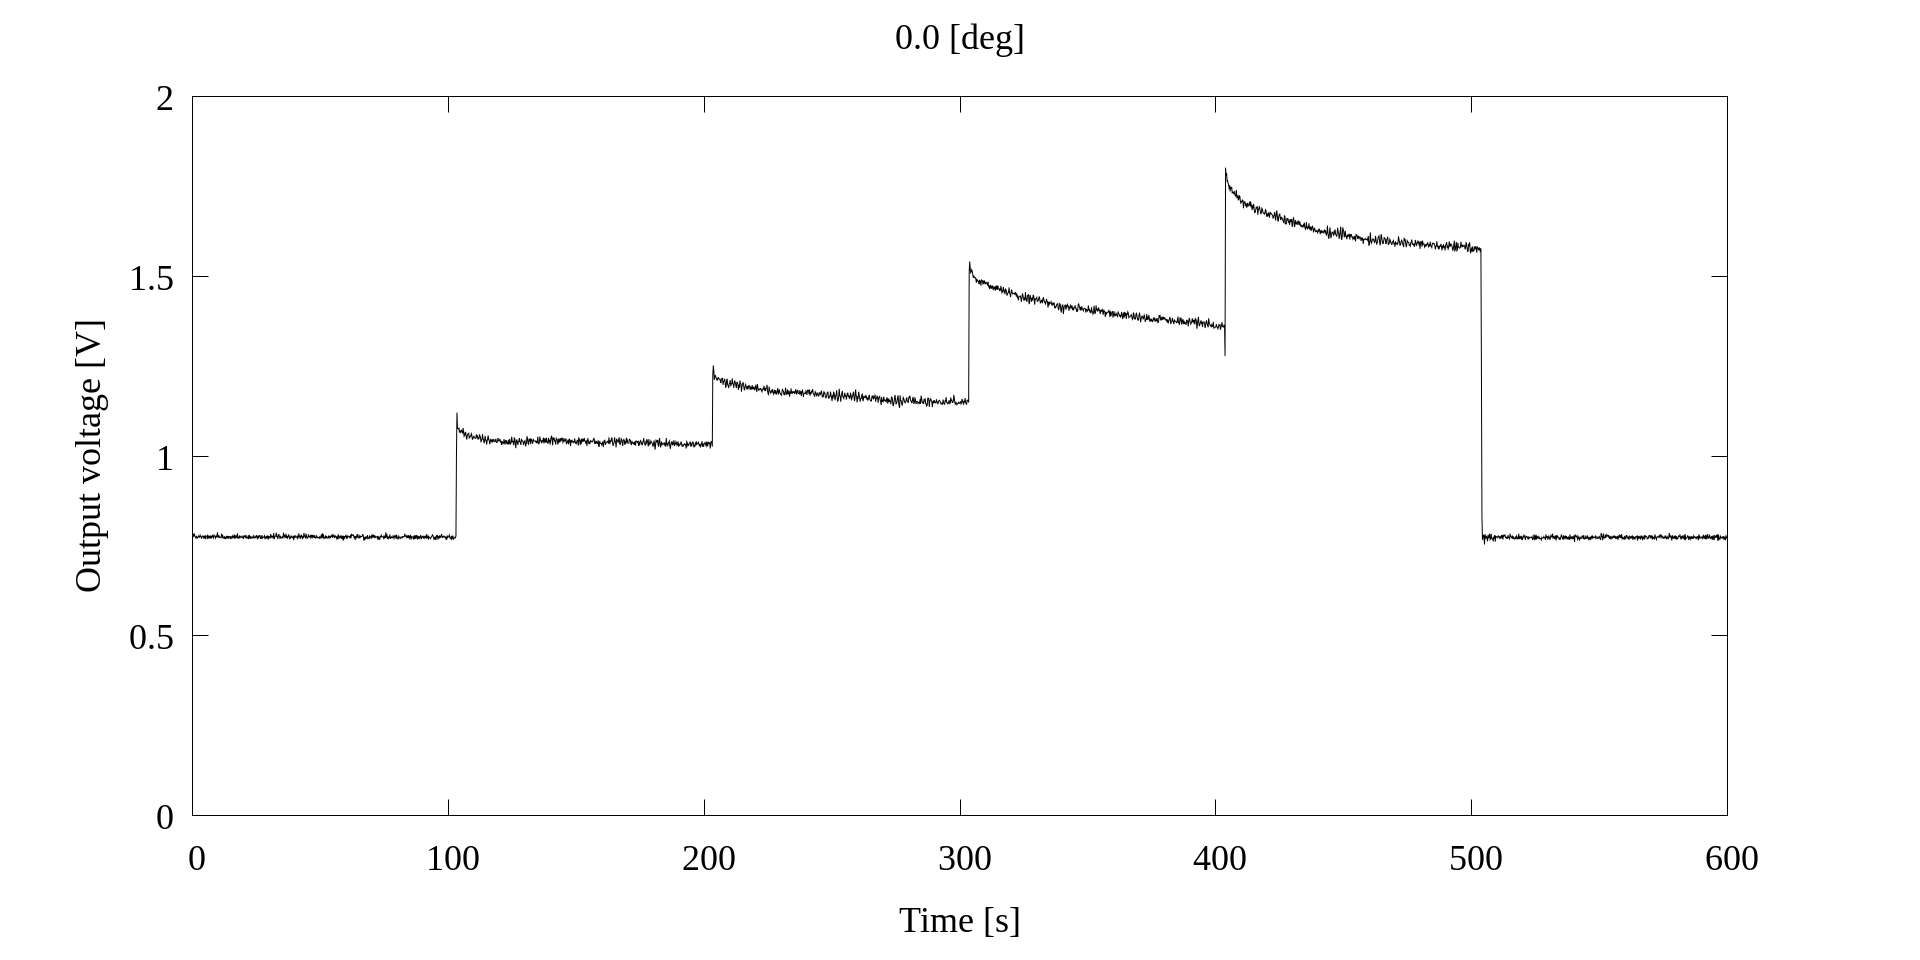
\includegraphics[width=95mm]{../../02_workspace/result/2-1/plot/01-1_loadcell/01_loadcell_0.png}
        \caption{Loadcell output voltage : 0 [deg] (1st)}
    \end{center}
\end{figure}

実験は,4.4.3測定手順に沿って行われているため,すべての実験結果は時間経過による変化は同様の形となる.
また,100秒周期でロードセルの押込距離を変化させていることがわかる.
このとき,ドリフト補正についてはFig.における測定開始直後および測定終了直前のデータを用いて行う.
はじめに,測定開始直後100秒間のデータから以下の手順に沿って平均値を算出する.

\begin{enumerate}[(1)]
    \item 測定開始後,60秒間(150点)の待機時間のデータを除く
    \item 待機時刻終了直後およびロードセルの動作直前のそれぞれ5秒間(25点)を除いた計30秒間(150点)のデータの平均値を計算する
    \item [※] なお,前後5秒間の計10秒間[50点]のデータを除くのは,
          データロガーの測定開始と自動ステージの動作プログラムの始動は
          人為的に同期させるため,その時刻のズレを除くためである.
    \item その平均値は測定時刻の中央に位置し,算出された2点を結ぶことで補正直線を算出する.
    \item 実験結果と算出された補正直線の差を取ることで,ドリフト補正を行うことができる.
\end{enumerate}

以下のFig.に,ドリフト補正を適用した結果を示す,

\begin{figure}[htbp]
    \footnotesize
    \begin{center}
        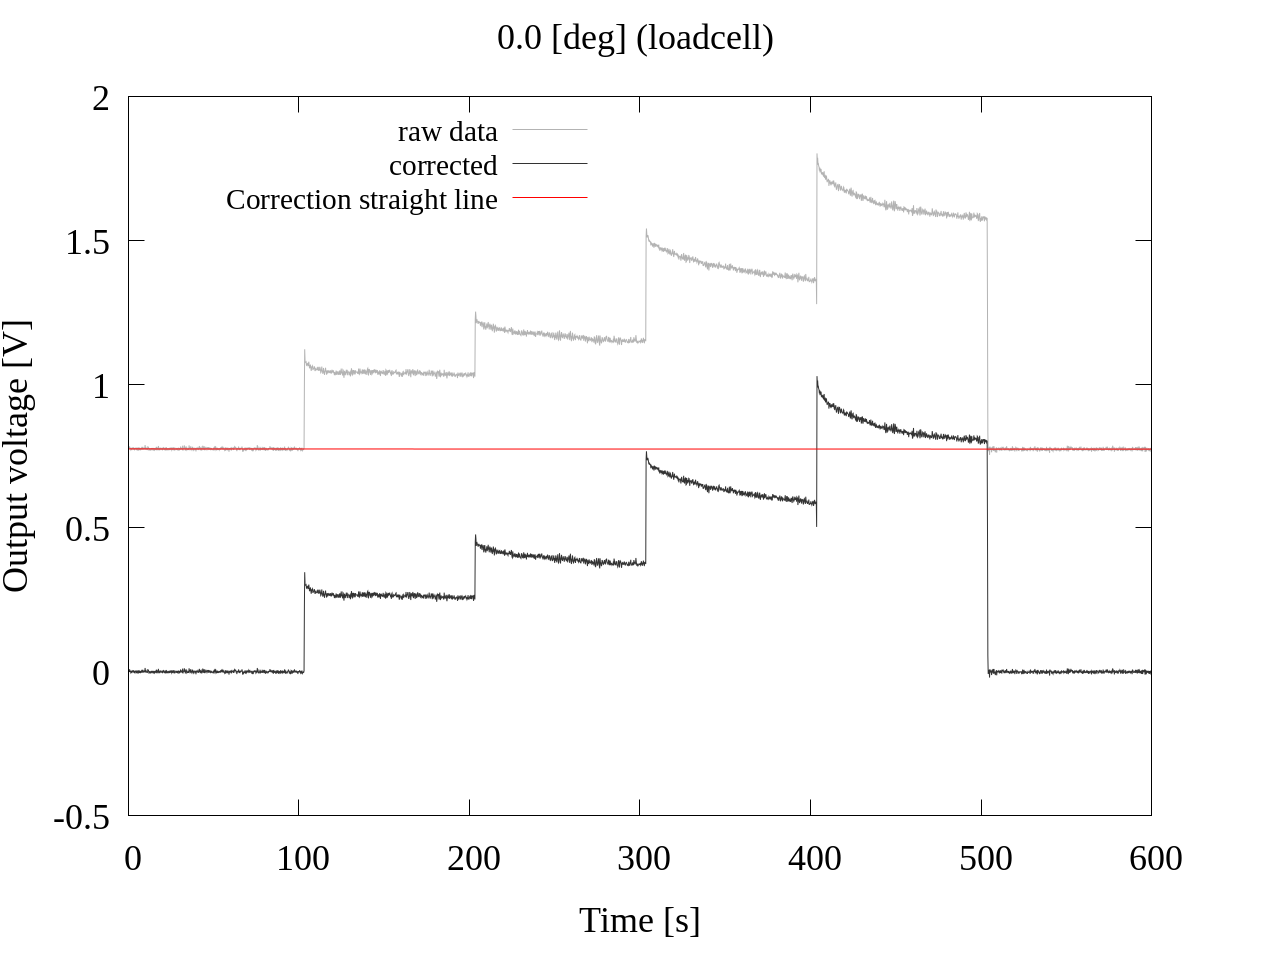
\includegraphics[width=95mm]{../../02_workspace/result/2-1/plot/02-1_loadcell/02_loadcell-drift_0.png}
        \caption{Drift correction : 0 [deg] (1st)}
    \end{center}
\end{figure}

Fig.をみると,ロードセルの出力電圧の持つオフセットは補正直線によって取り除かれていることがわかる.

\subsubsection{押込距離における平均値の算出}

次に各押込距離ごとの平均値を算出する.
算出する方法は,ドリフト補正時に使用した平均値の算出方法を各押込距離の結果に適用することで求めることとする.

以下のFig.に,算出した平均値について示す.

\begin{figure}[htbp]
    \footnotesize
    \begin{center}
        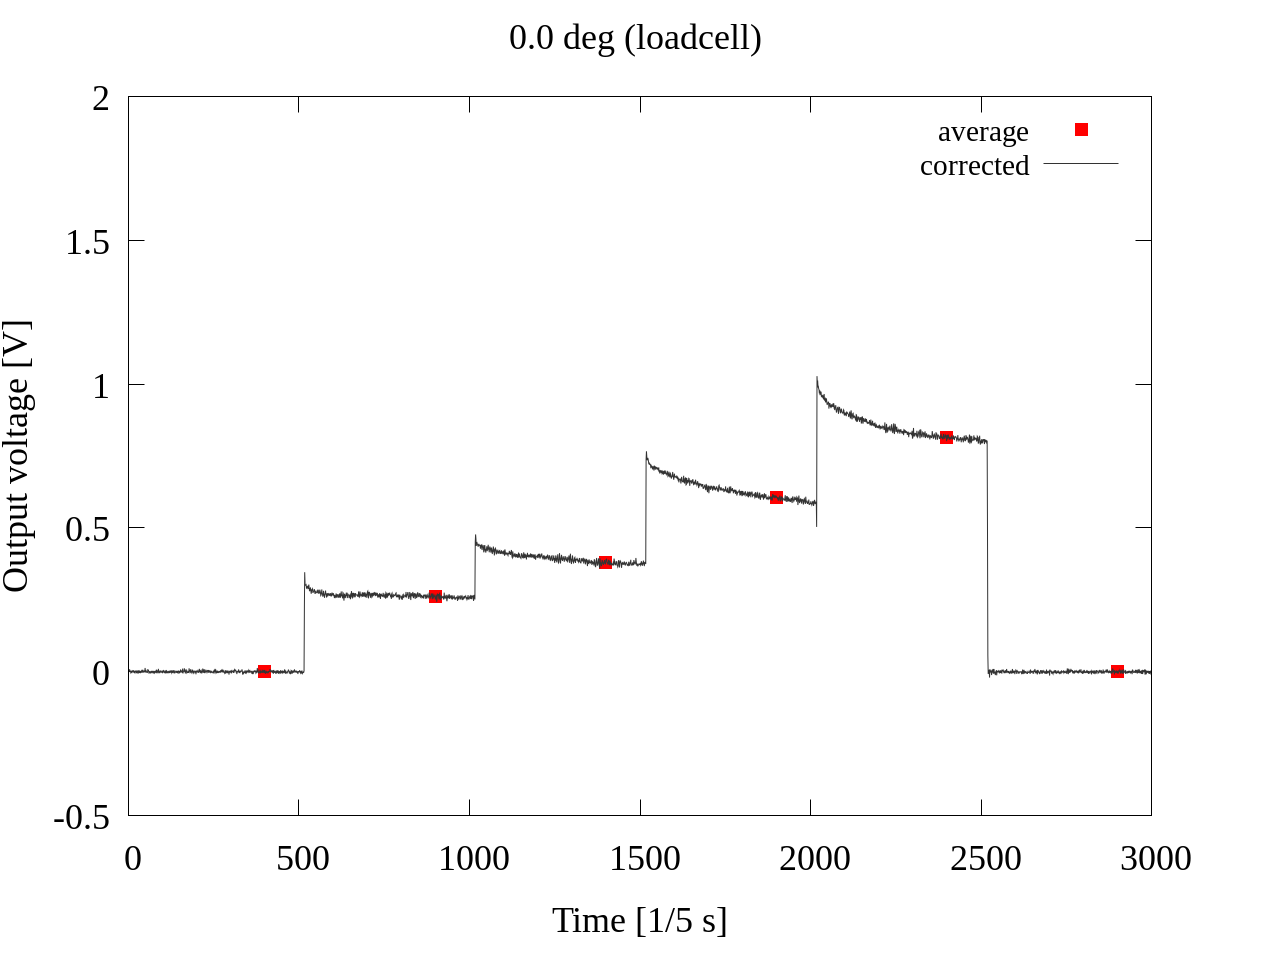
\includegraphics[width=95mm]{../../02_workspace/result/2-1/plot/03-1_loadcell/03_loadcell_average_0.png}
        \caption{Average of loadcell voltage : 0 [deg] (1st)}
    \end{center}
\end{figure}

また,この操作を各押込角度の実験結果に適用する.

\newpage

また,以下のFig.,Fig,に実験1回目,0[deg]における抗力方向および揚力方向のひずみセンサの出力電圧についての
平均値算出結果を示す.

\begin{multicols}{2}
    \begin{figure_here}
        \begin{center}
            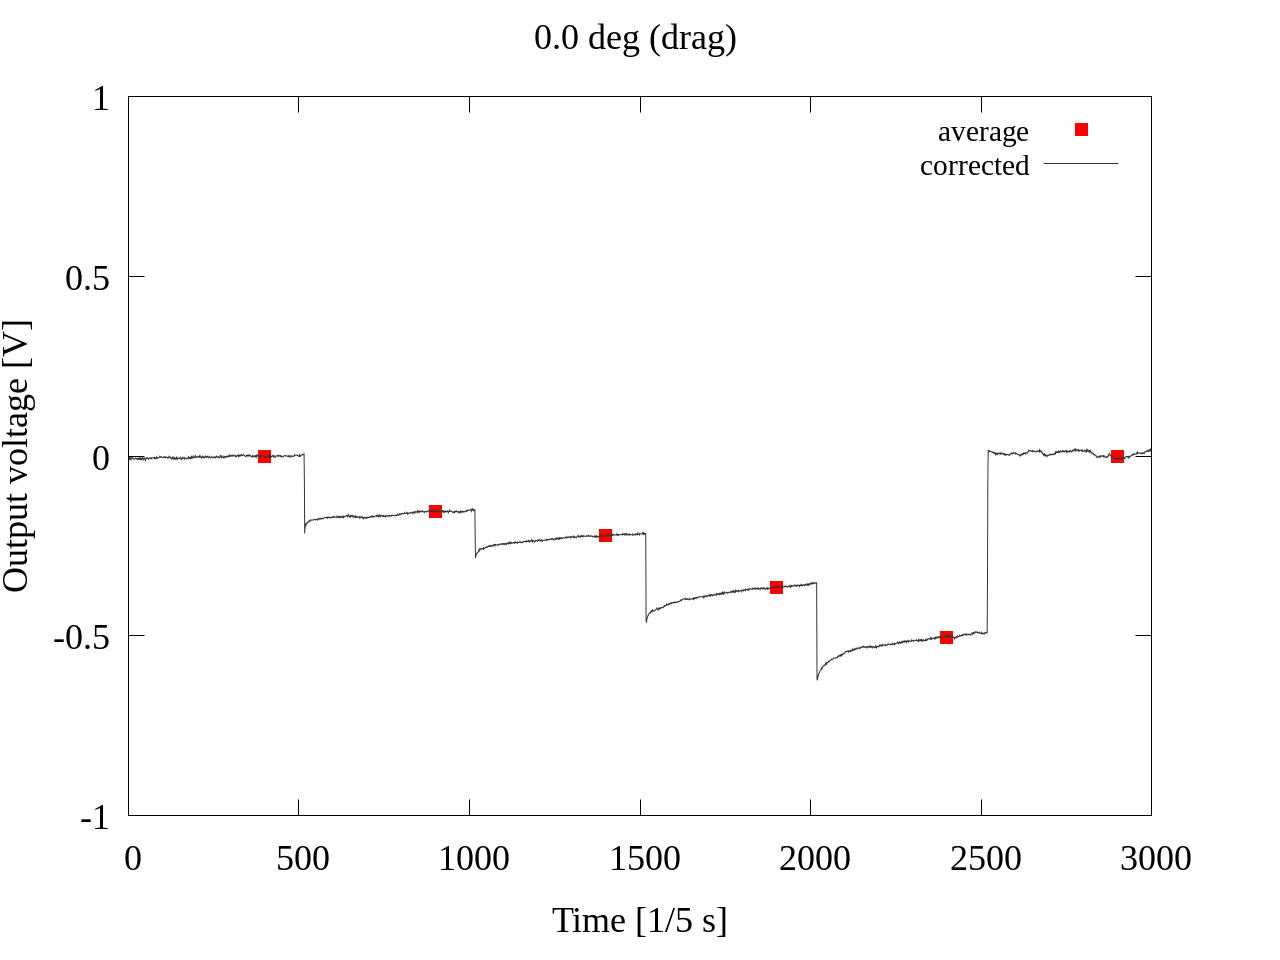
\includegraphics[width=65mm]{../../02_workspace/result/2-1/plot/03-2_drag/03_drag_average_0.png}
            \caption{Average of drag voltage: 0 [deg] (1st)}
            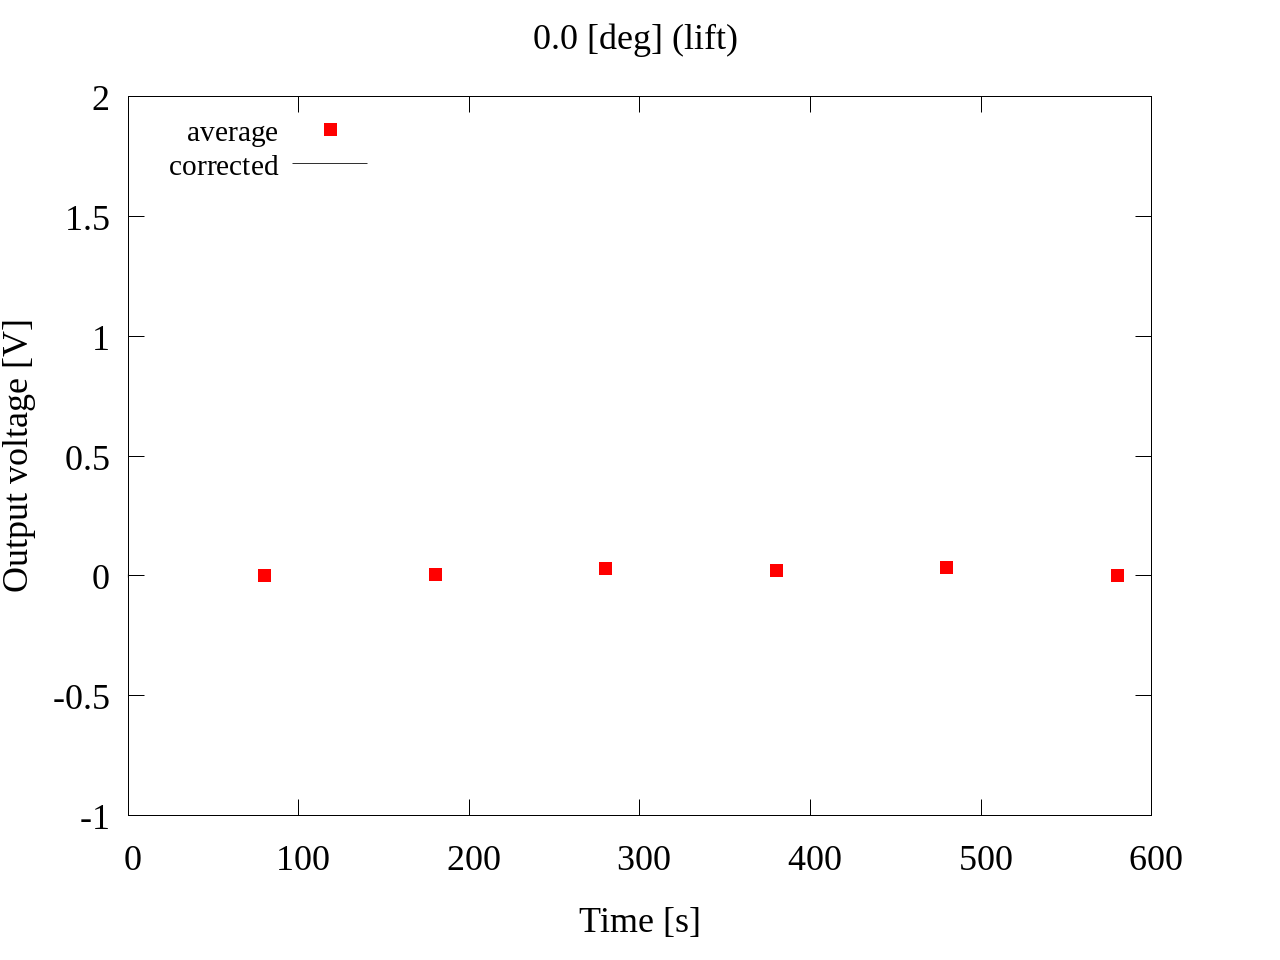
\includegraphics[width=65mm]{../../02_workspace/result/2-1/plot/03-3_lift/03_lift_average_0.png}
            \caption{Average of lift voltage: 0 [deg] (1st)}
        \end{center}
    \end{figure_here}
\end{multicols}

\newpage

\subsubsection{出力電圧勾配の算出}

算出された平均値を用いて,出力電圧勾配を求める.
使用する平均値は5つ目までのデータであり,
ロードセルの出力電圧$V$とひずみセンサの出力電圧$V_d$,$V_l$は各押込距離ごとのデータを持つ行列となるため,
ロードセルの出力電圧行列を$v_i$,ひずみセンサの出力電圧行列の抗力方向を$V_{di}$,揚力方向を$V_{li}$とする
($i = 1, 2, 3, 4, 5$).
ここで,ロードセルと抗力方向のひずみセンサの対応するデータの組を$(V_i,V_{di})$,
ロードセルと抗力方向のひずみセンサの対応するデータの組を$(V_i,V_{li})$として,
最小二乗法を用いてそれぞれの傾きを求める.
このとき,その傾きについて出力電圧勾配と定義し,抗力方向を$v_d$,揚力方向を$v_l$とする.

\begin{eqnarray}
    \displaystyle v_d &= \frac{n\sum^n_{k=1} V_{k} V_{dk} - \sum^n_{k=1} V_{K} \sum^n_{K=1} V_{dk}}{n\sum^n_{k=1}V_{dk}^2 - \left(\sum^n_{k=1}V_k\right)^2}\\
    \displaystyle v_l &= \frac{n\sum^n_{k=1} V_{k} V_{lk} - \sum^n_{k=1} V_{K} \sum^n_{K=1} V_{lk}}{n\sum^n_{k=1}V_{lk}^2 - \left(\sum^n_{k=1}V_k\right)^2}
\end{eqnarray}

Fig.~Fig.に算出した出力電圧勾配についての結果を示す.
なお,示している結果は1回目の実験結果である.

\begin{multicols}{2}
    \begin{figure_here}
        \begin{center}
            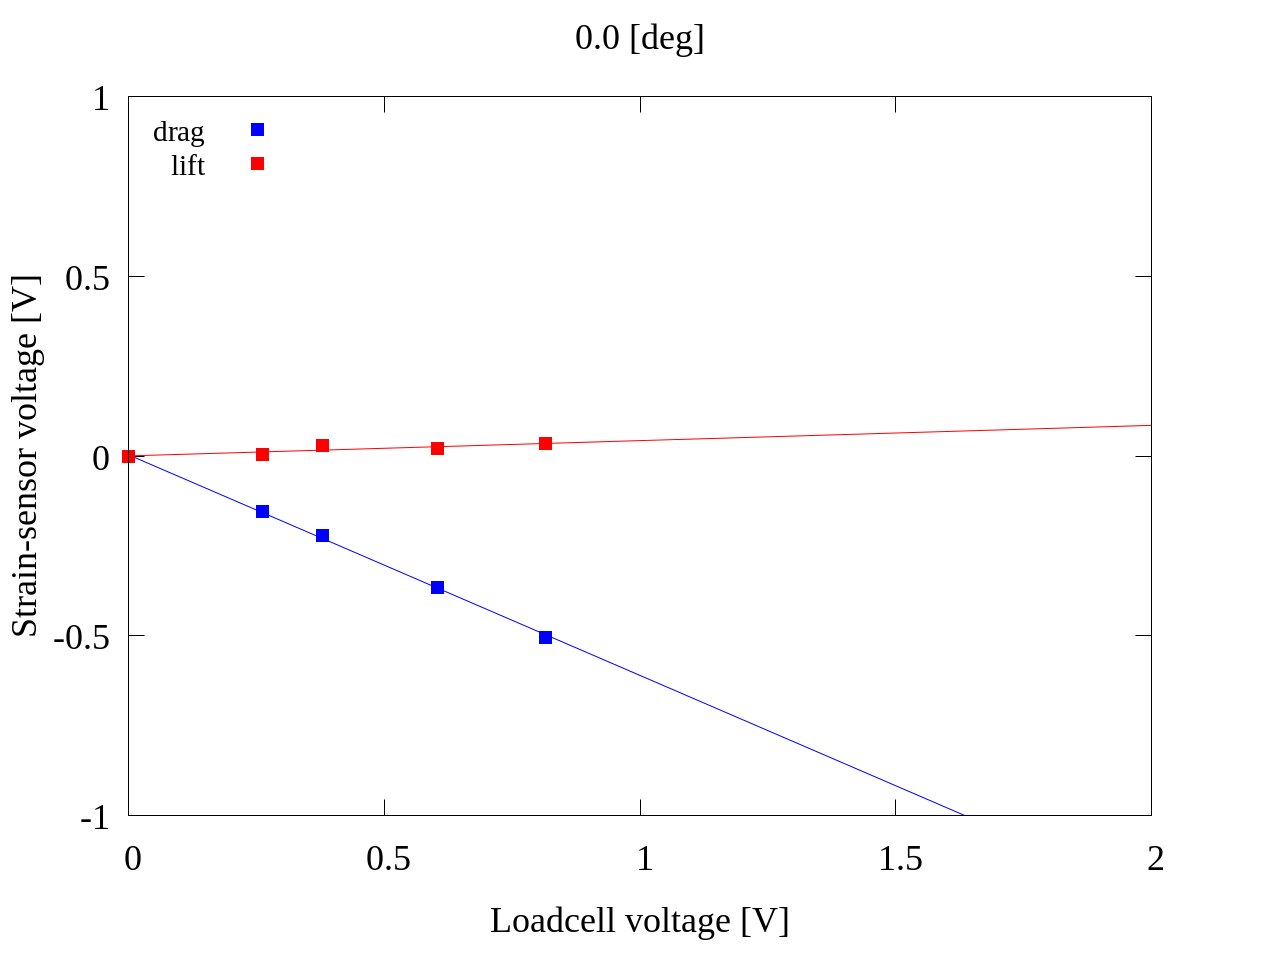
\includegraphics[width=70mm]{../../02_workspace/result/2-1/plot/04/04_linear_0.png}
            \caption{Gradient of output voltage : 0 [deg]}
            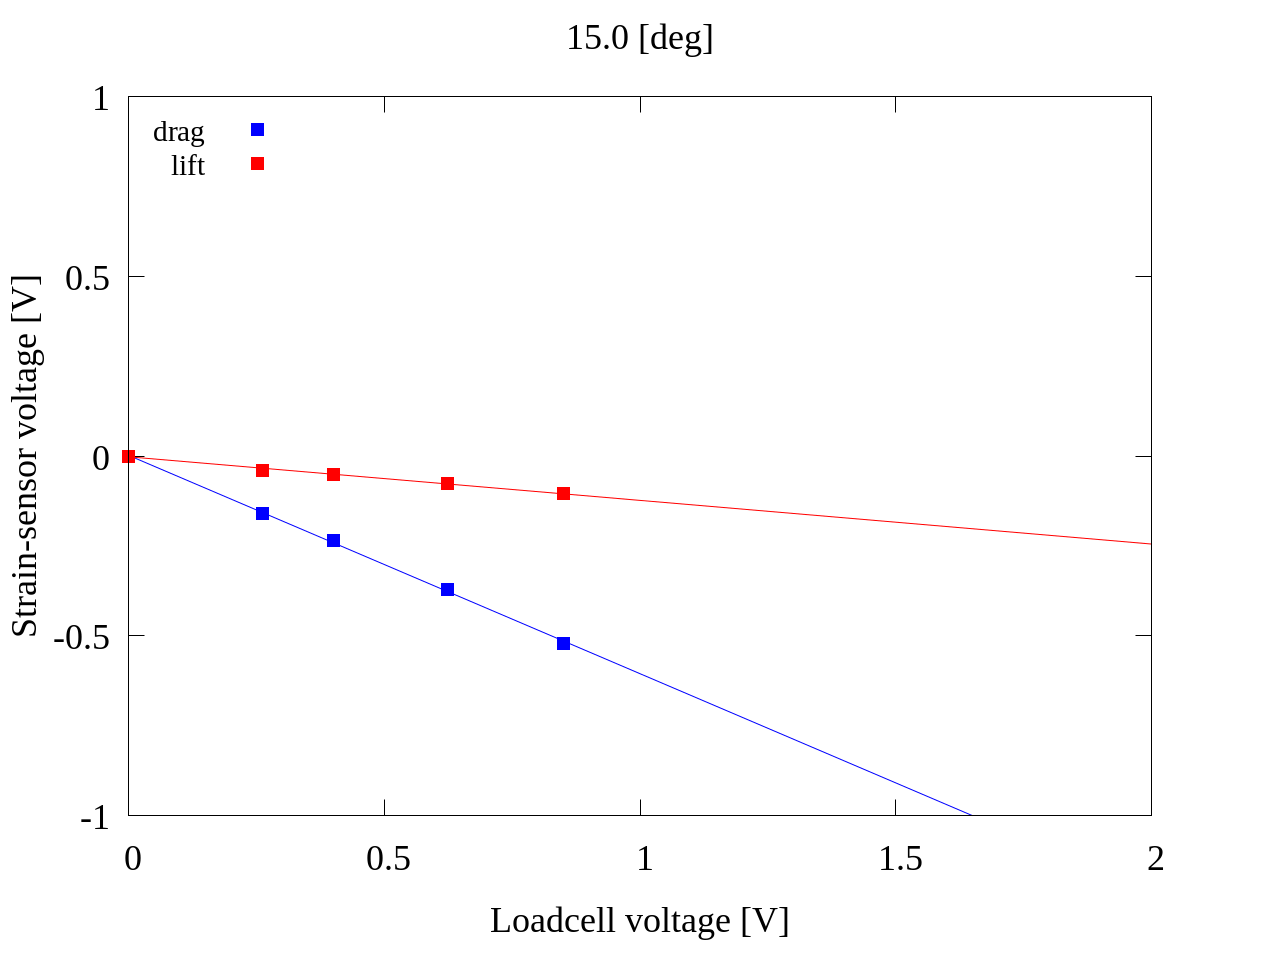
\includegraphics[width=70mm]{../../02_workspace/result/2-1/plot/04/04_linear_150.png}
            \caption{Gradient of output voltage : 15 [deg]}
            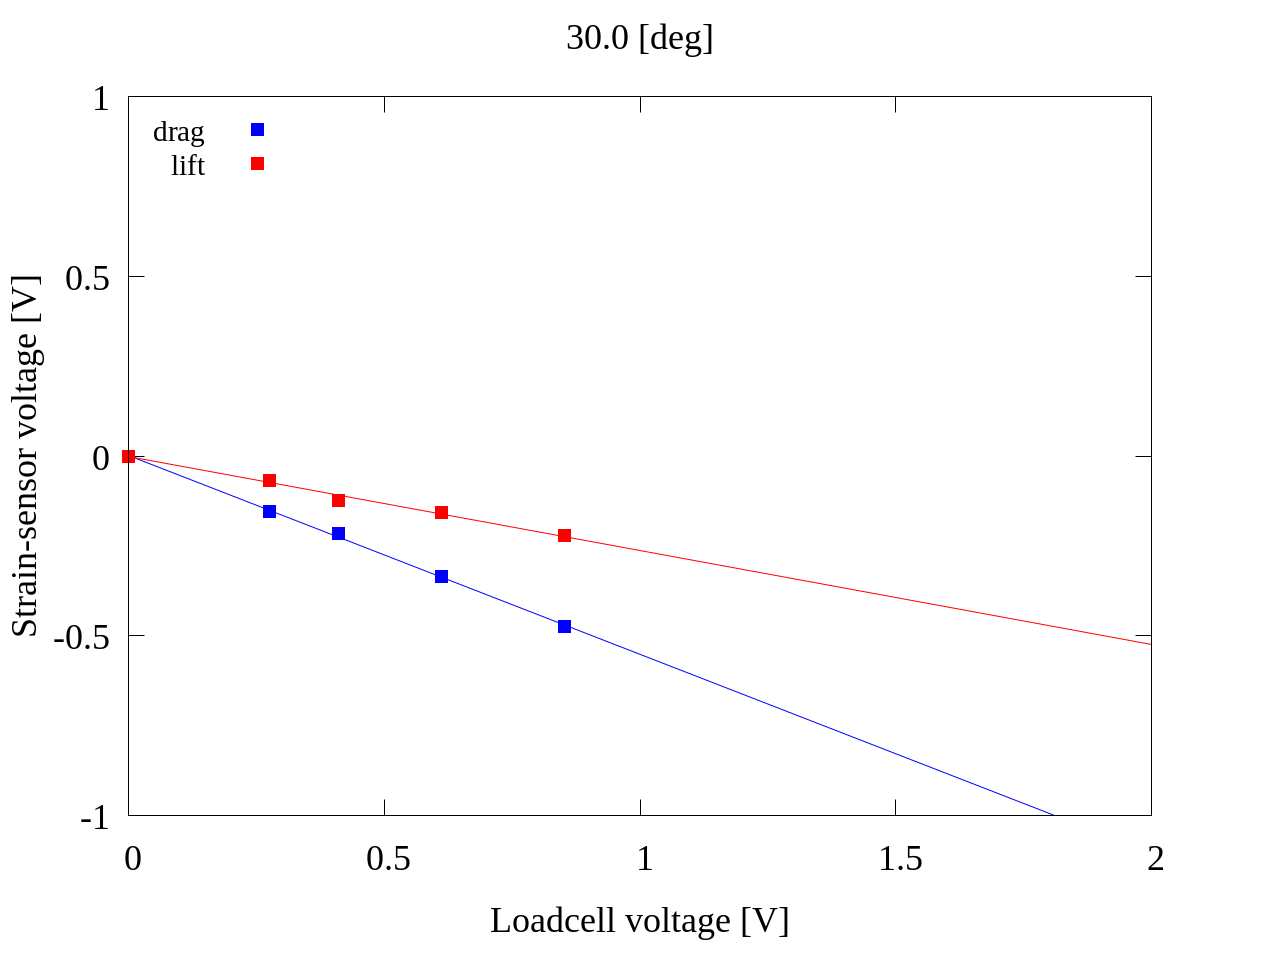
\includegraphics[width=70mm]{../../02_workspace/result/2-1/plot/04/04_linear_300.png}
            \caption{Gradient of output voltage : 30 [deg]}
            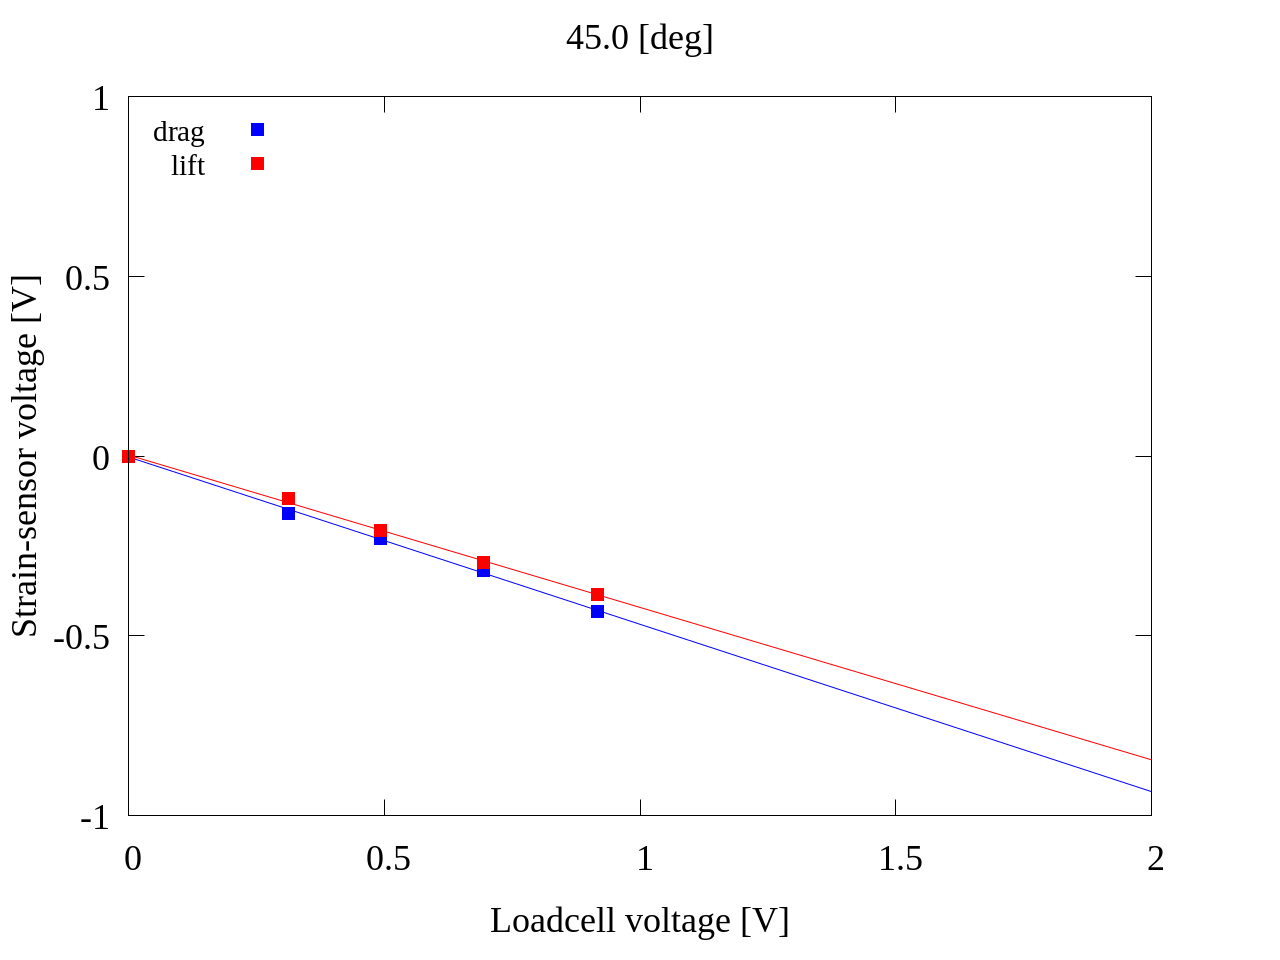
\includegraphics[width=70mm]{../../02_workspace/result/2-1/plot/04/04_linear_450.png}
            \caption{Gradient of output voltage : 45 [deg]}
            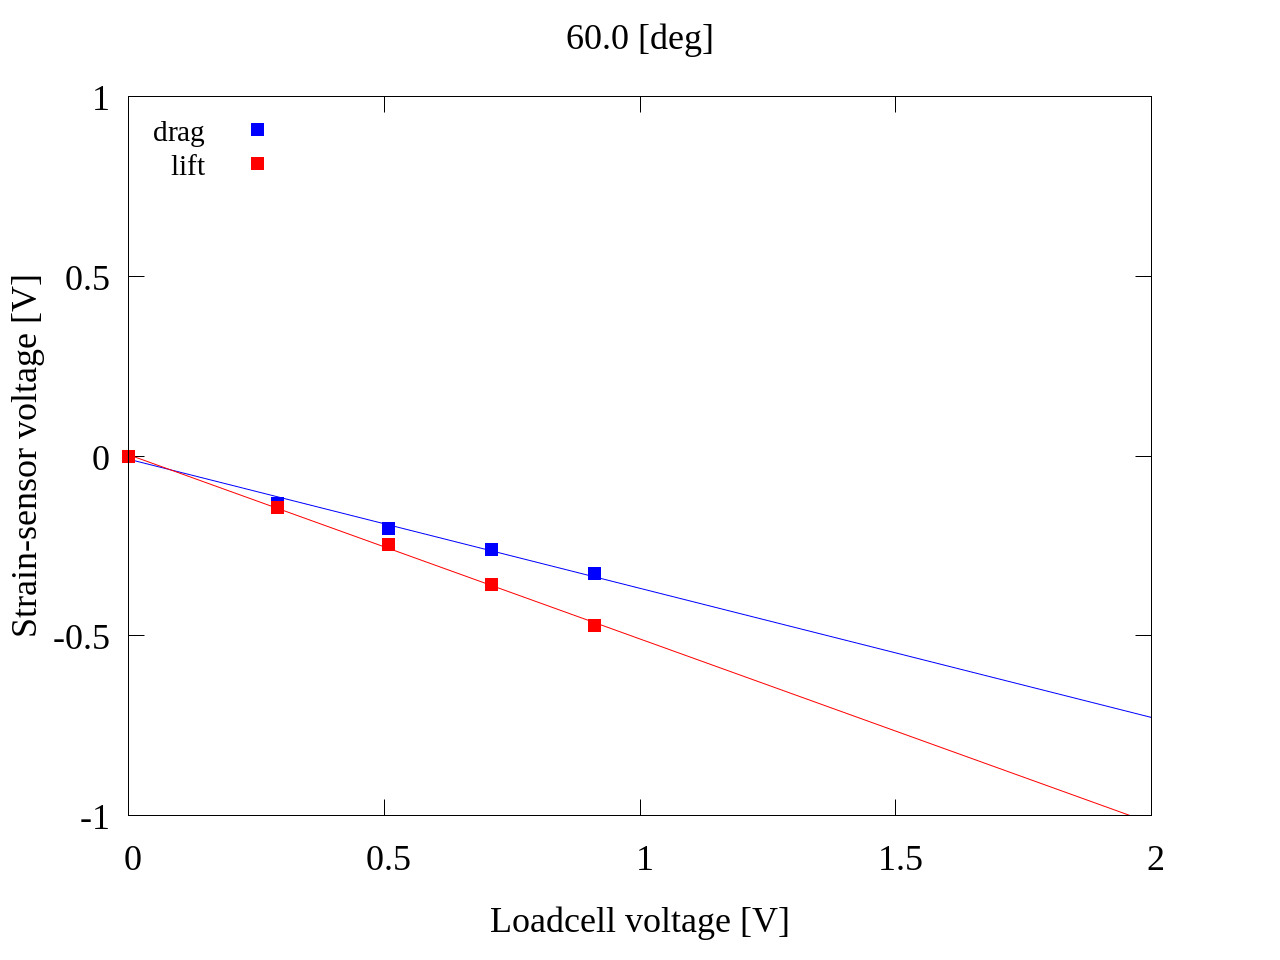
\includegraphics[width=70mm]{../../02_workspace/result/2-1/plot/04/04_linear_600.png}
            \caption{Gradient of output voltage : 60 [deg]}
            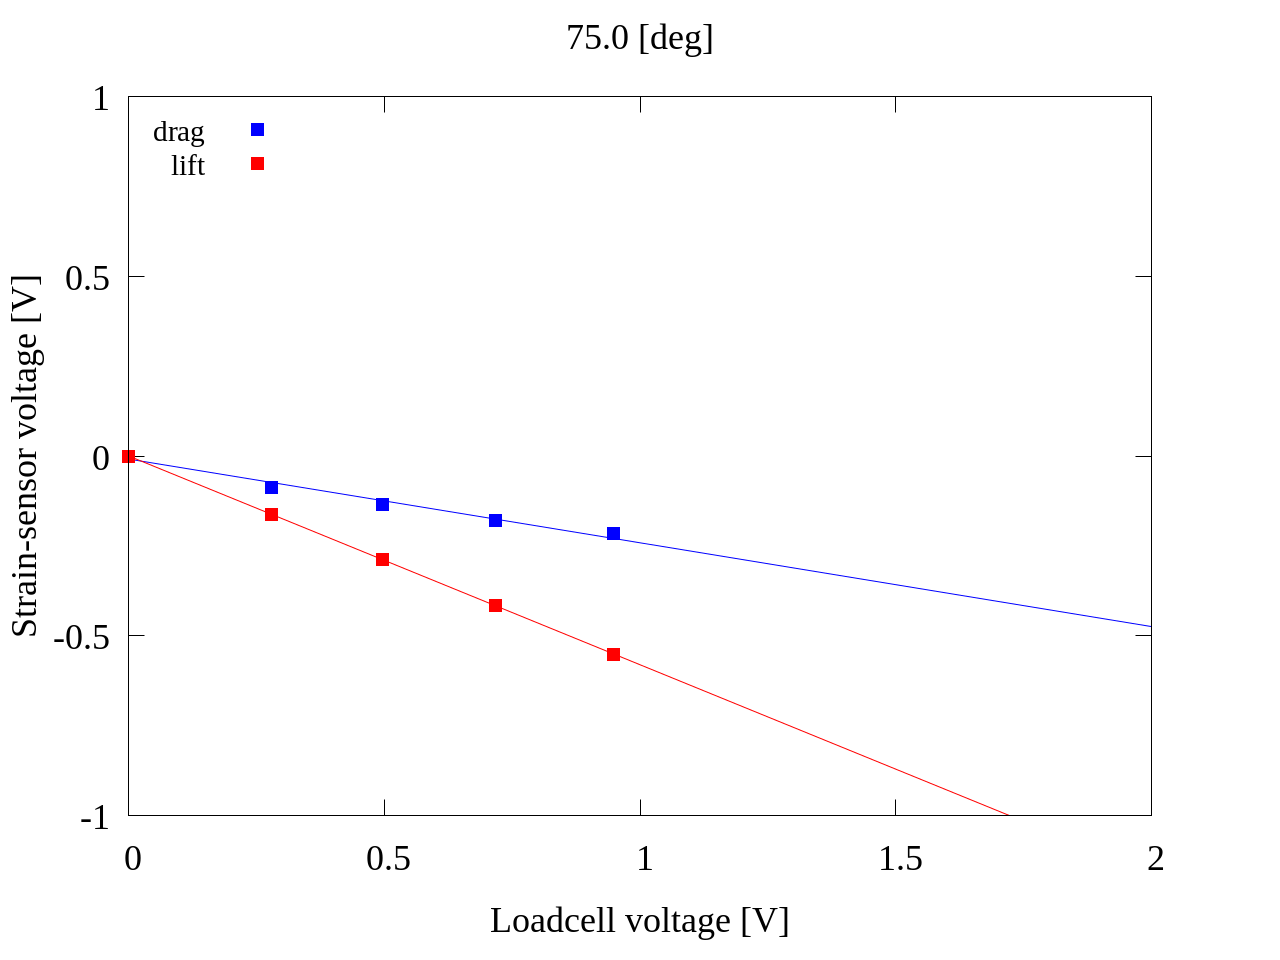
\includegraphics[width=70mm]{../../02_workspace/result/2-1/plot/04/04_linear_750.png}
            \caption{Gradient of output voltage : 75 [deg]}
            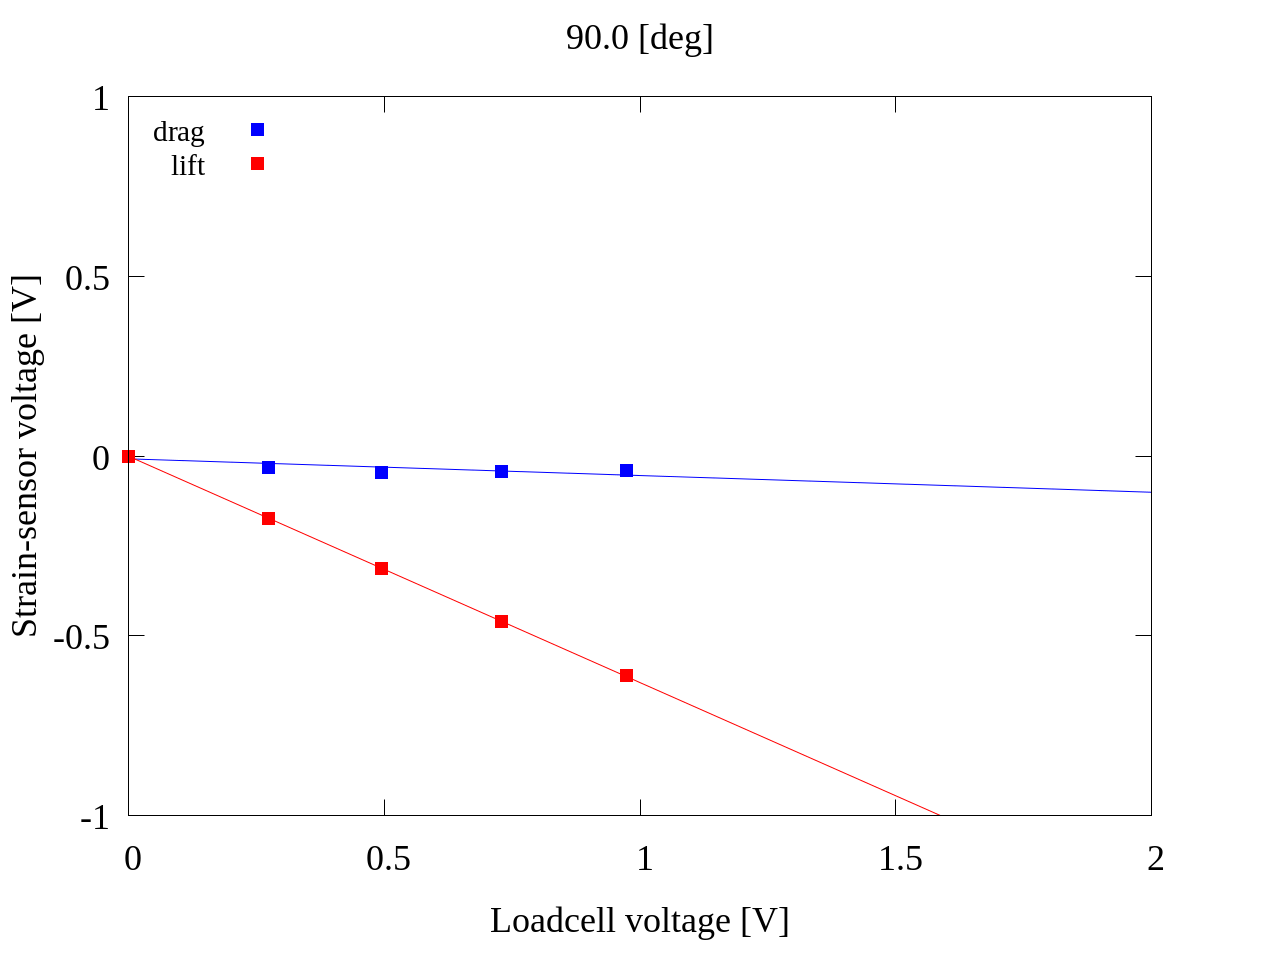
\includegraphics[width=70mm]{../../02_workspace/result/2-1/plot/04/04_linear_900.png}
            \caption{Gradient of output voltage : 90 [deg]}
            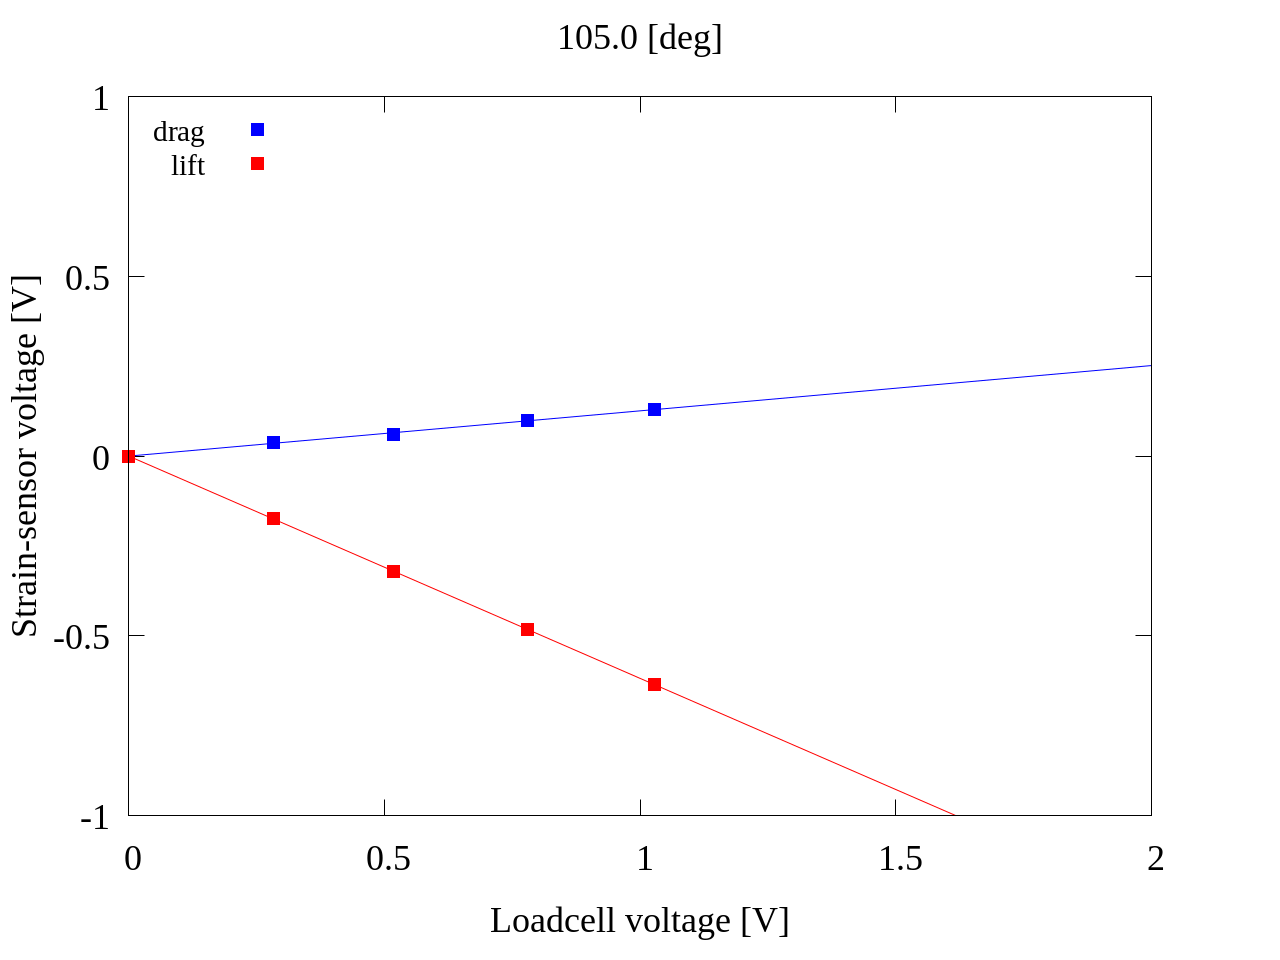
\includegraphics[width=70mm]{../../02_workspace/result/2-1/plot/04/04_linear_1050.png}
            \caption{Gradient of output voltage : 105 [deg]}
            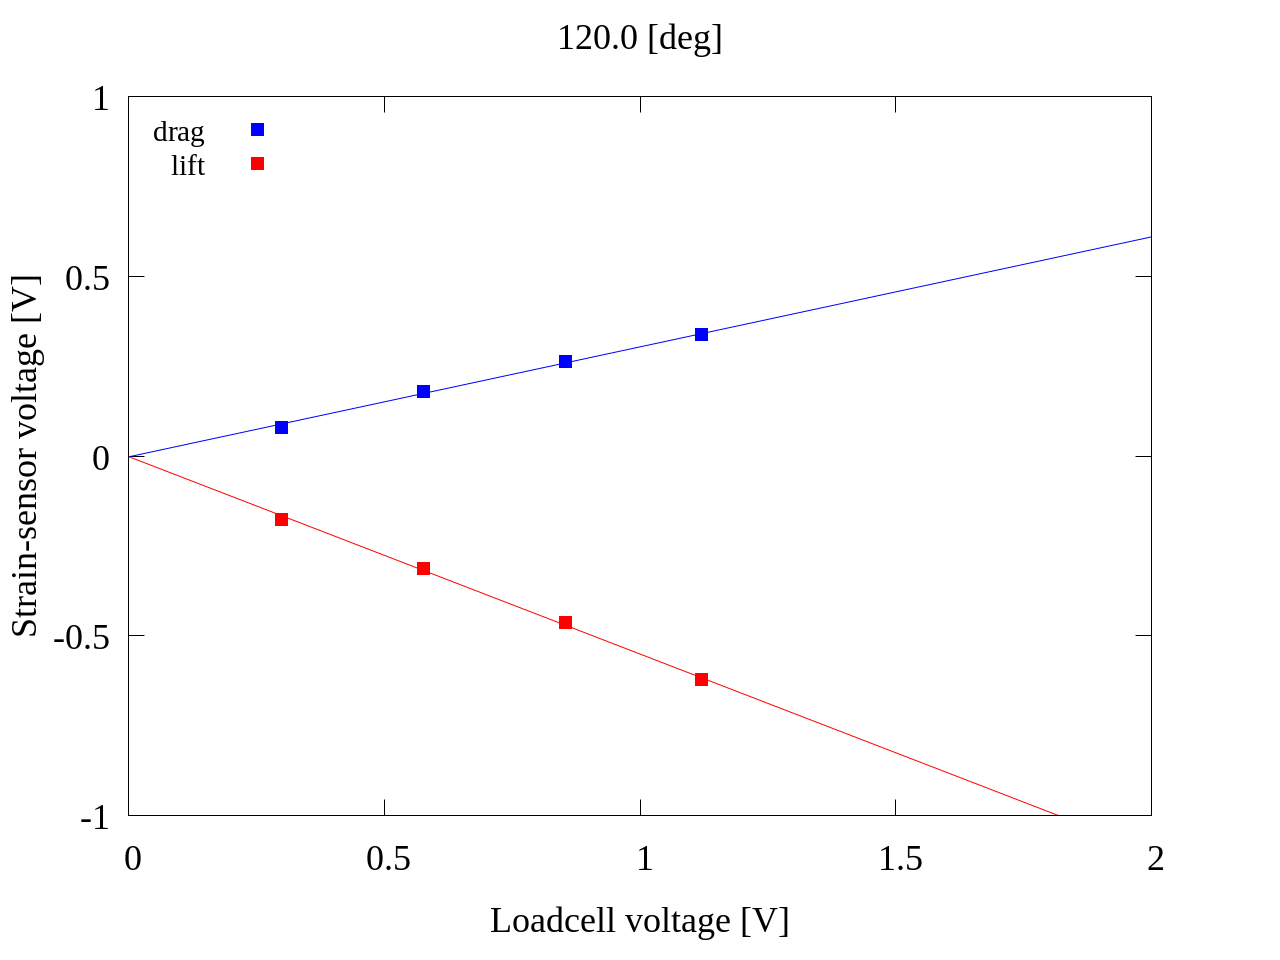
\includegraphics[width=70mm]{../../02_workspace/result/2-1/plot/04/04_linear_1200.png}
            \caption{Gradient of output voltage : 120 [deg]}
            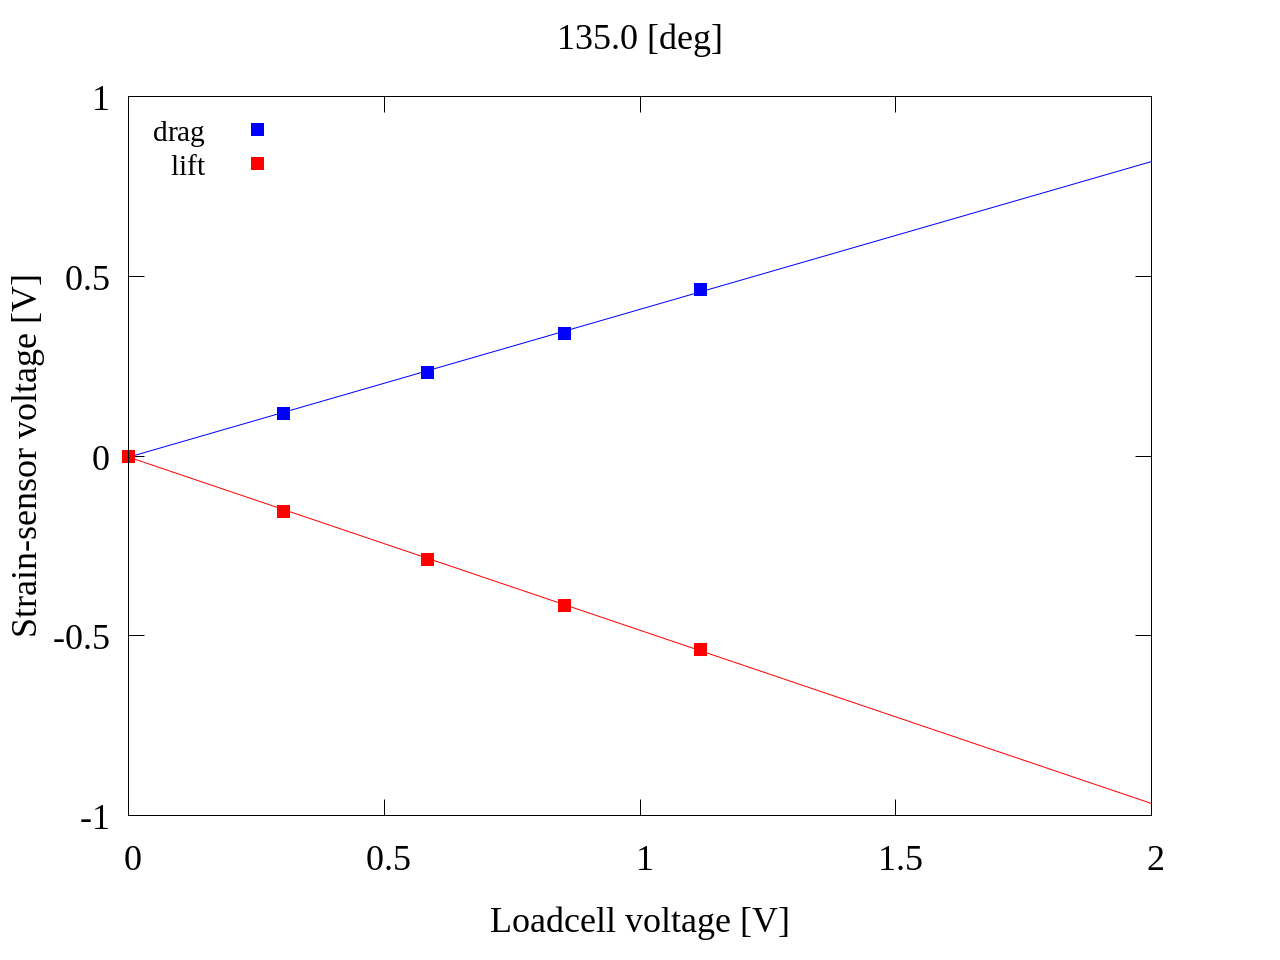
\includegraphics[width=70mm]{../../02_workspace/result/2-1/plot/04/04_linear_1350.png}
            \caption{Gradient of output voltage : 135 [deg]}
            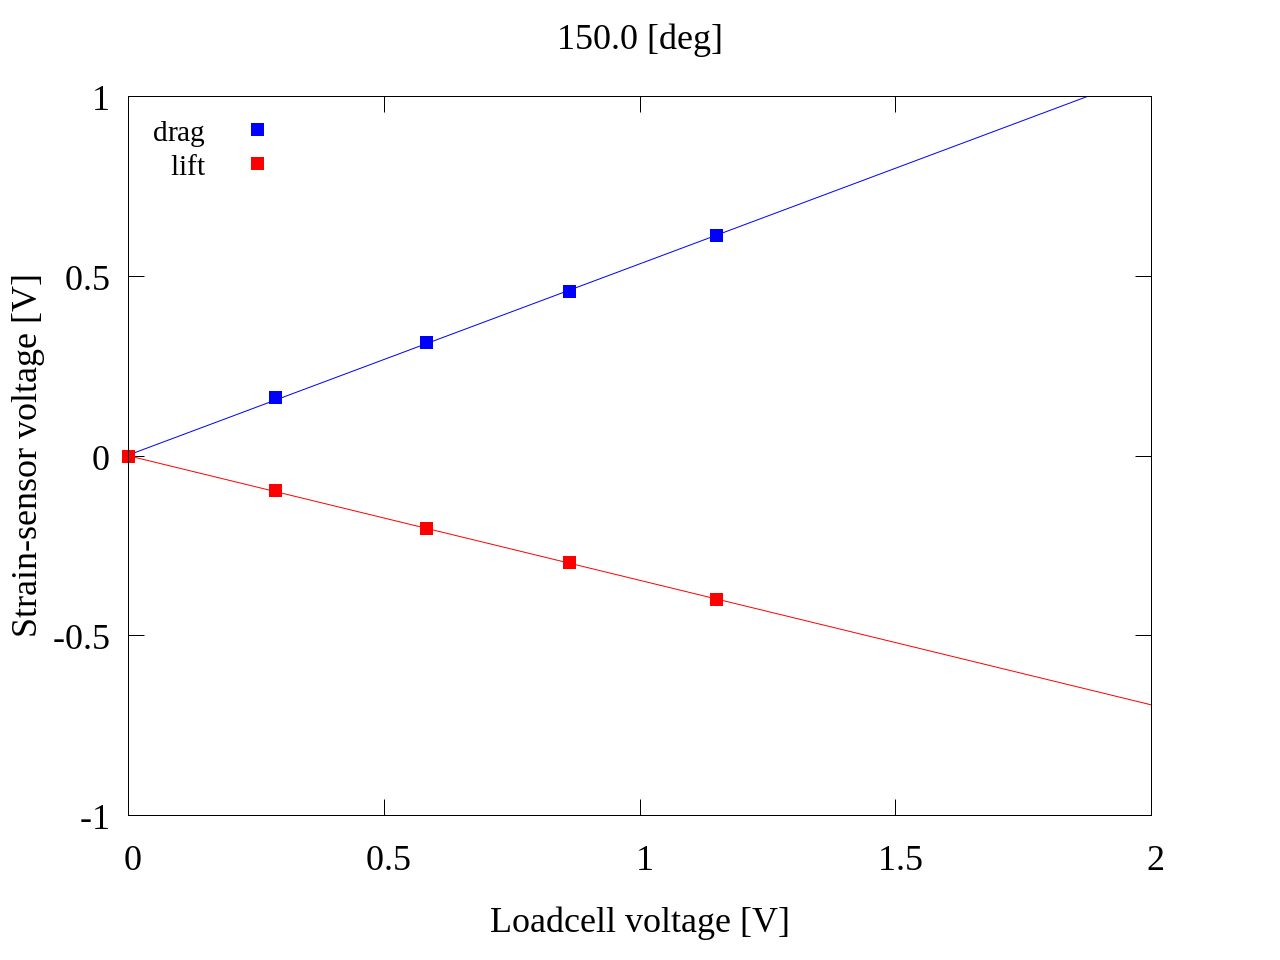
\includegraphics[width=70mm]{../../02_workspace/result/2-1/plot/04/04_linear_1500.png}
            \caption{Gradient of output voltage : 150 [deg]}
            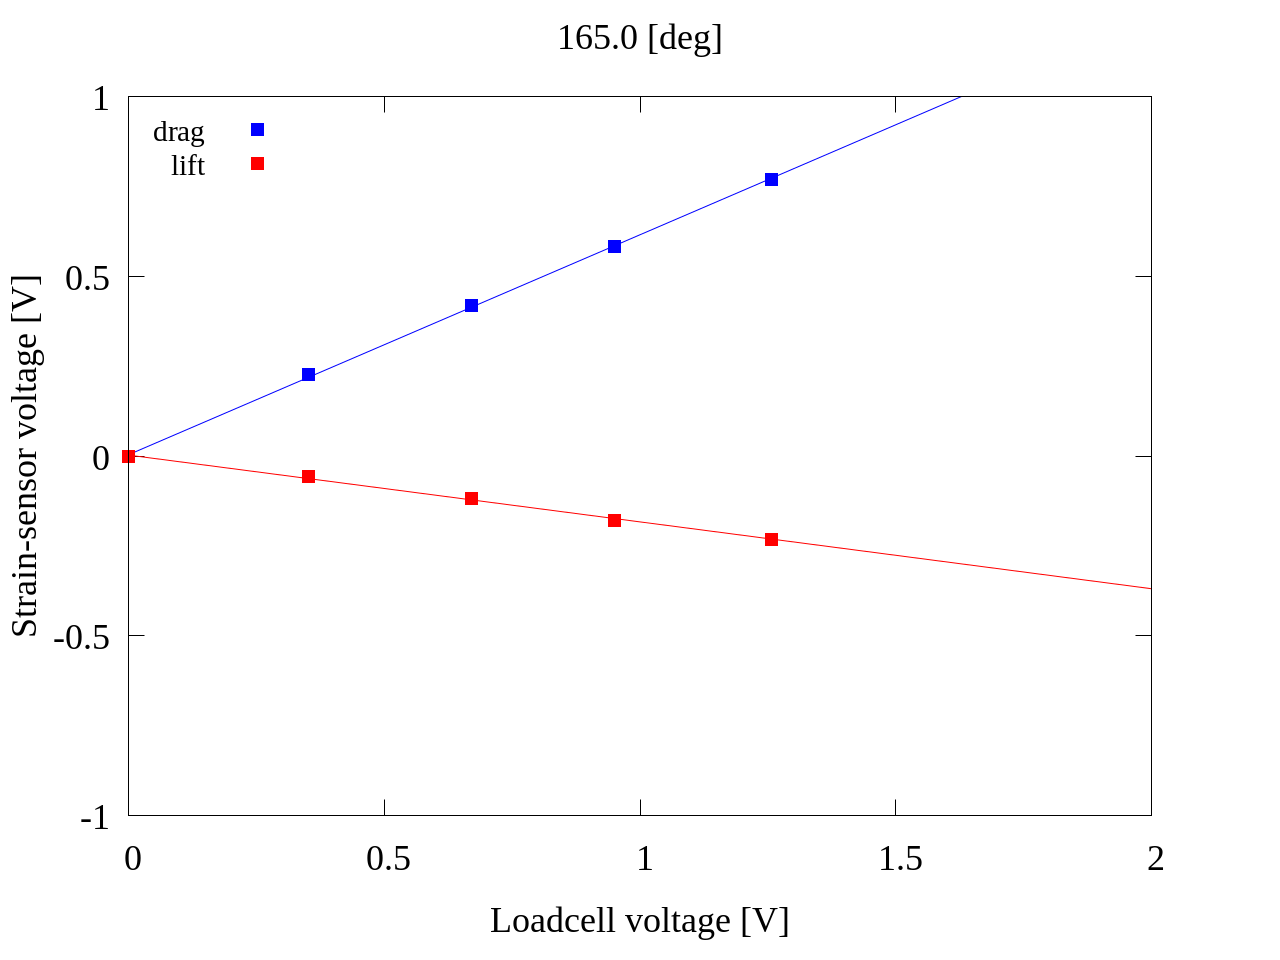
\includegraphics[width=70mm]{../../02_workspace/result/2-1/plot/04/04_linear_1650.png}
            \caption{Gradient of output voltage : 165 [deg]}
            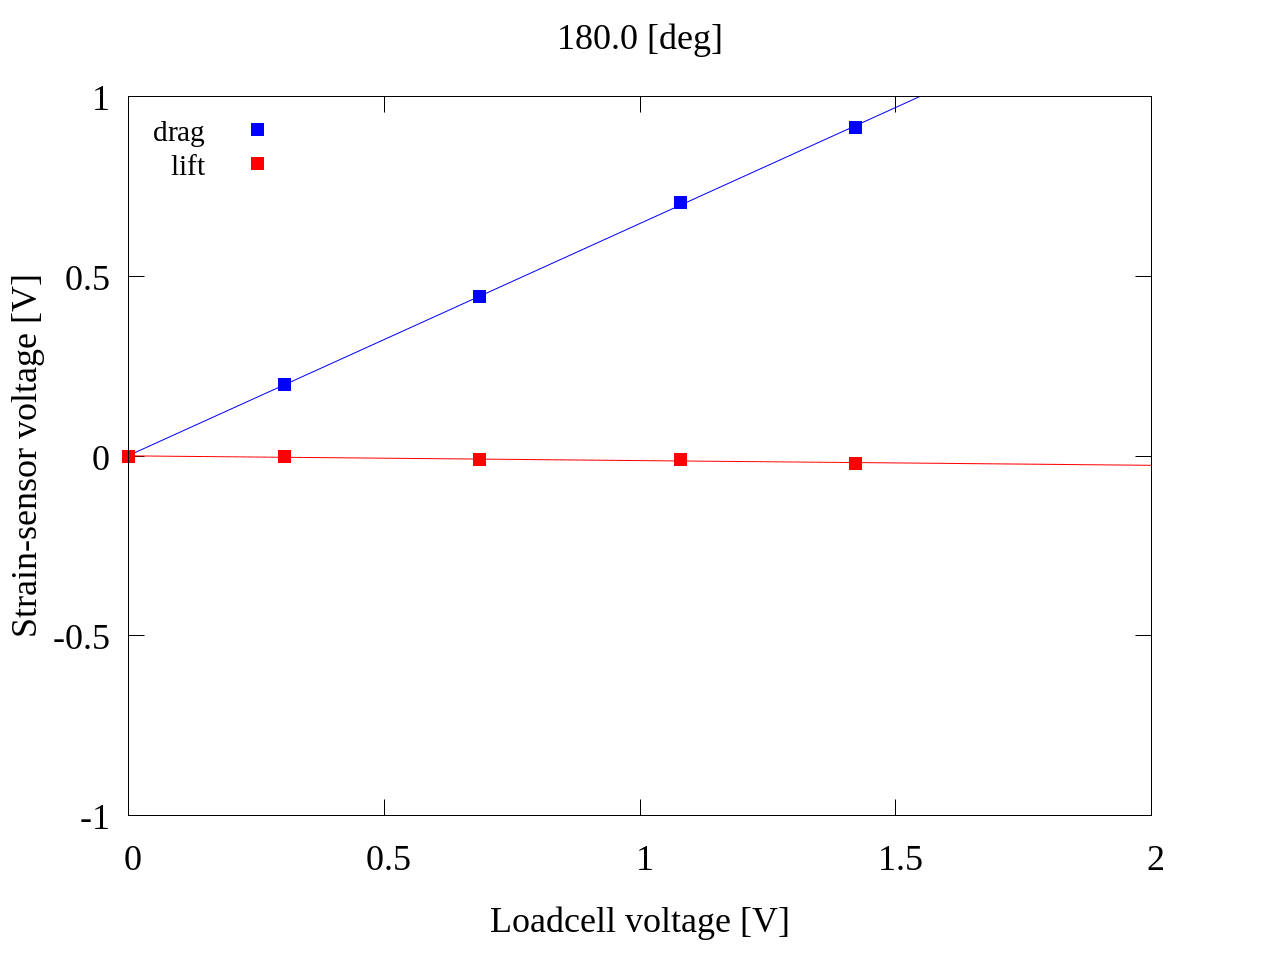
\includegraphics[width=70mm]{../../02_workspace/result/2-1/plot/04/04_linear_1800.png}
            \caption{Gradient of output voltage : 180 [deg]}
            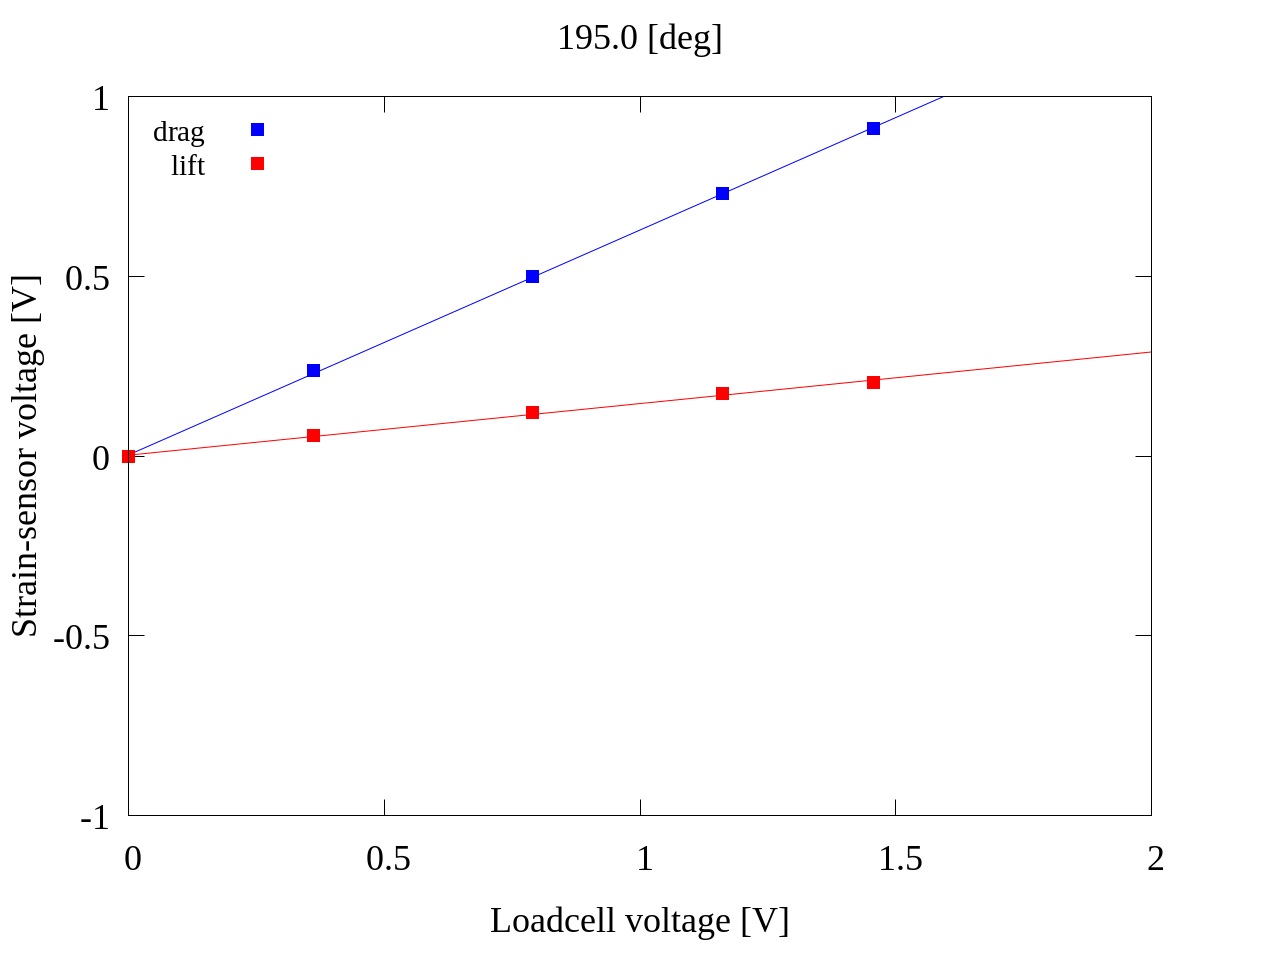
\includegraphics[width=70mm]{../../02_workspace/result/2-1/plot/04/04_linear_1950.png}
            \caption{Gradient of output voltage : 195 [deg]}
            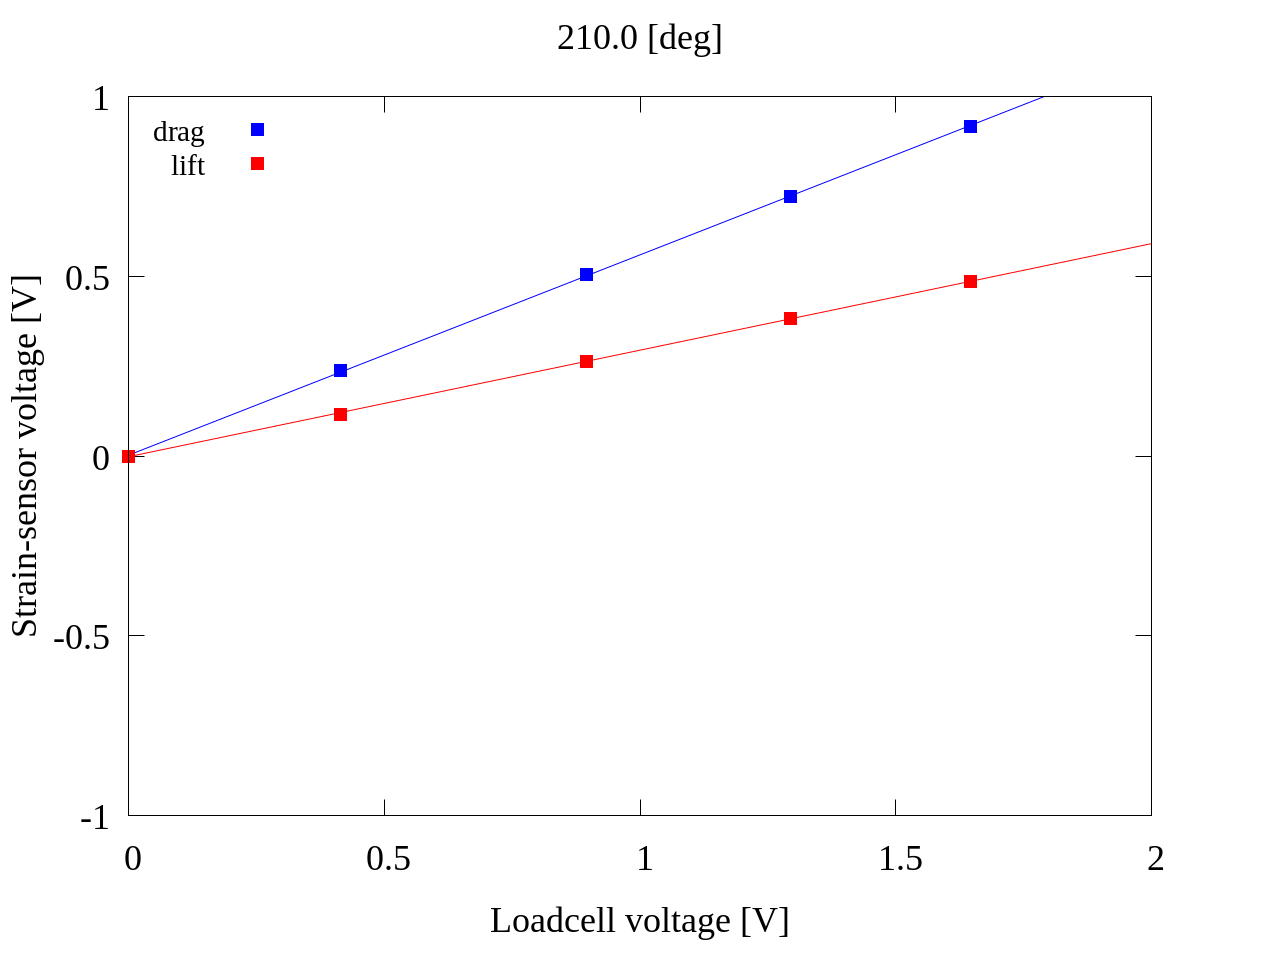
\includegraphics[width=70mm]{../../02_workspace/result/2-1/plot/04/04_linear_2100.png}
            \caption{Gradient of output voltage : 210 [deg]}
            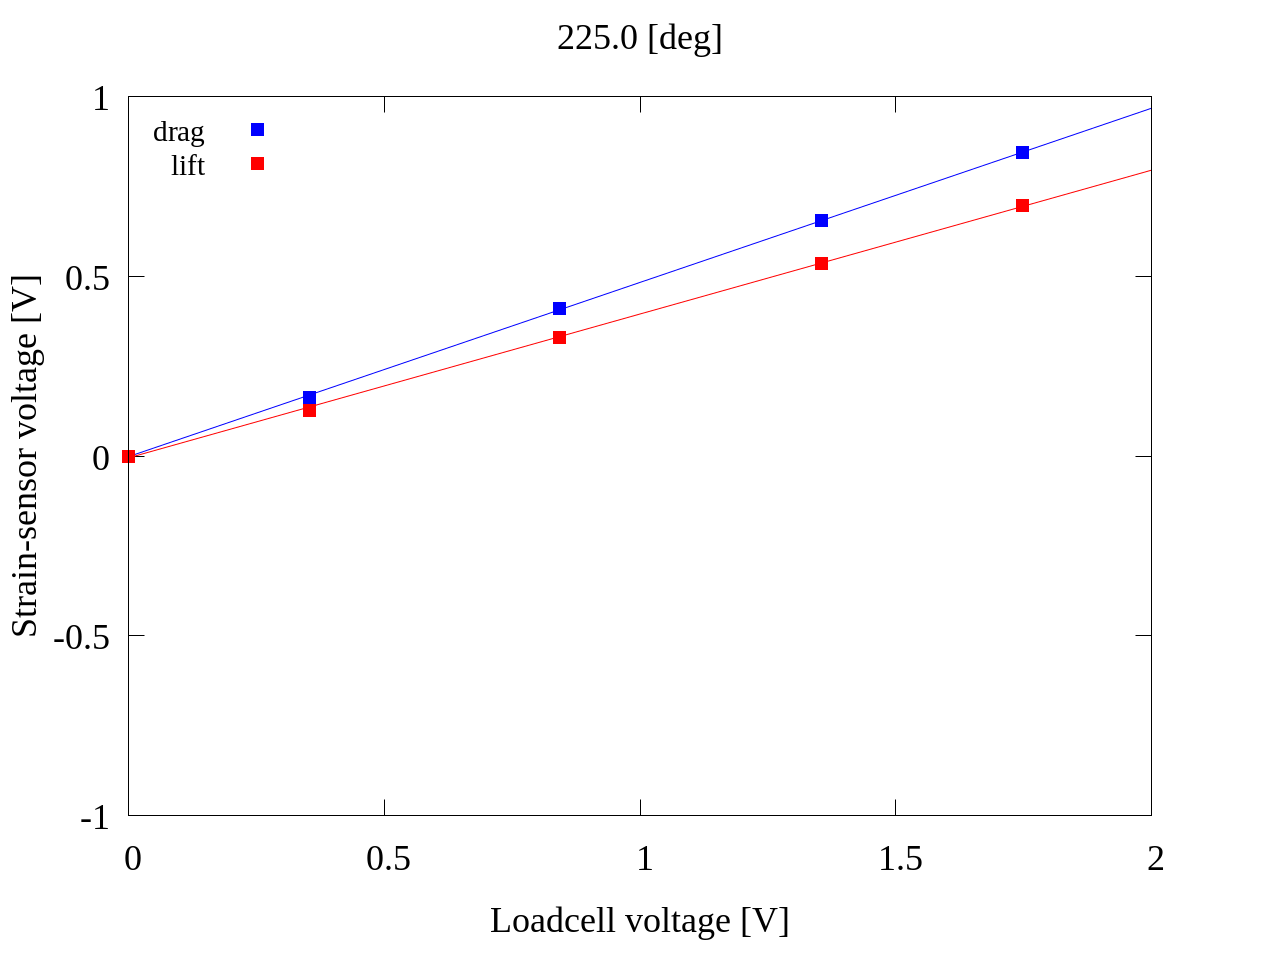
\includegraphics[width=70mm]{../../02_workspace/result/2-1/plot/04/04_linear_2250.png}
            \caption{Gradient of output voltage : 225 [deg]}
            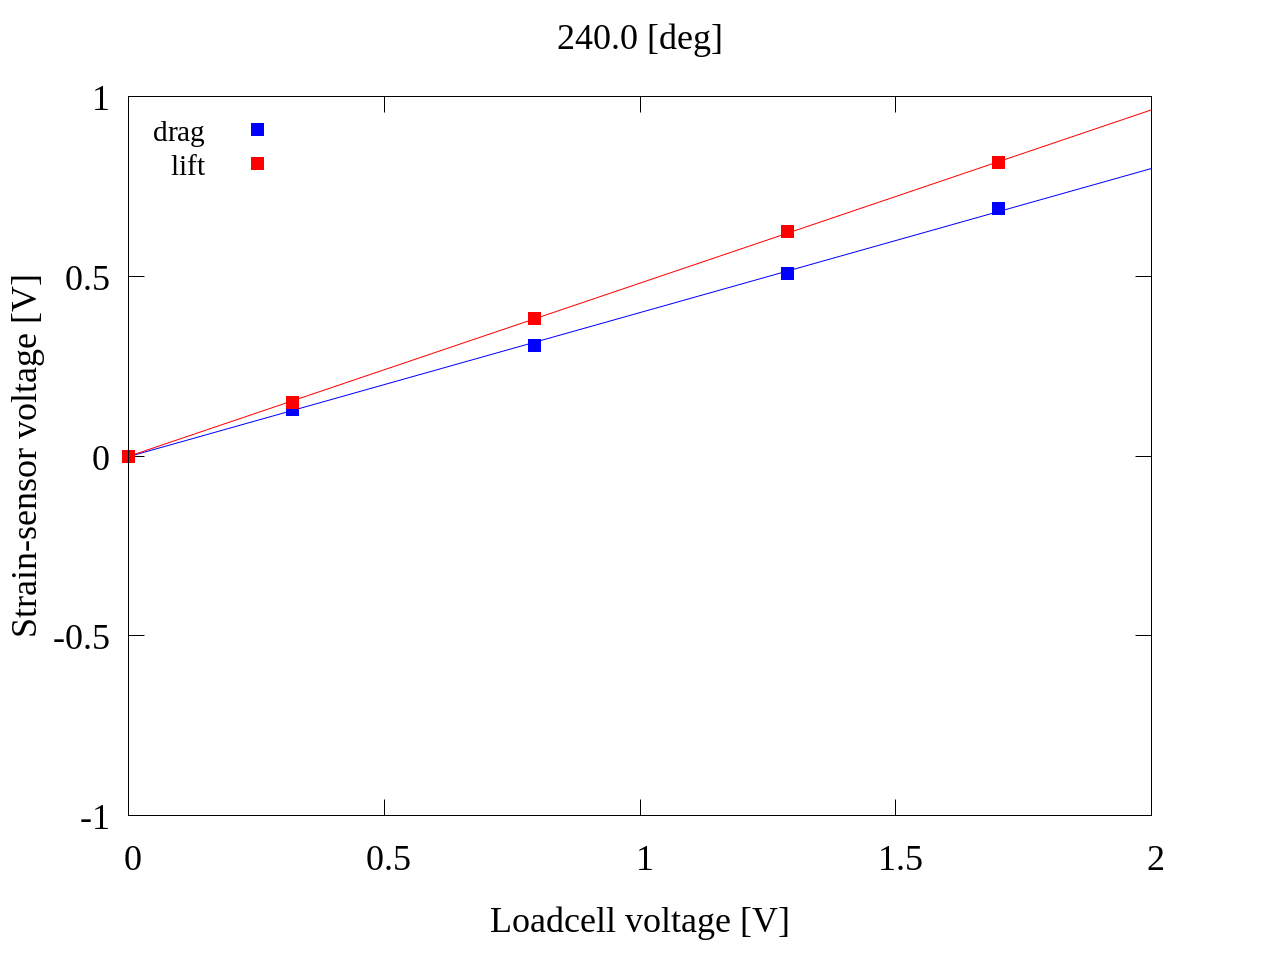
\includegraphics[width=70mm]{../../02_workspace/result/2-1/plot/04/04_linear_2400.png}
            \caption{Gradient of output voltage : 240 [deg]}
            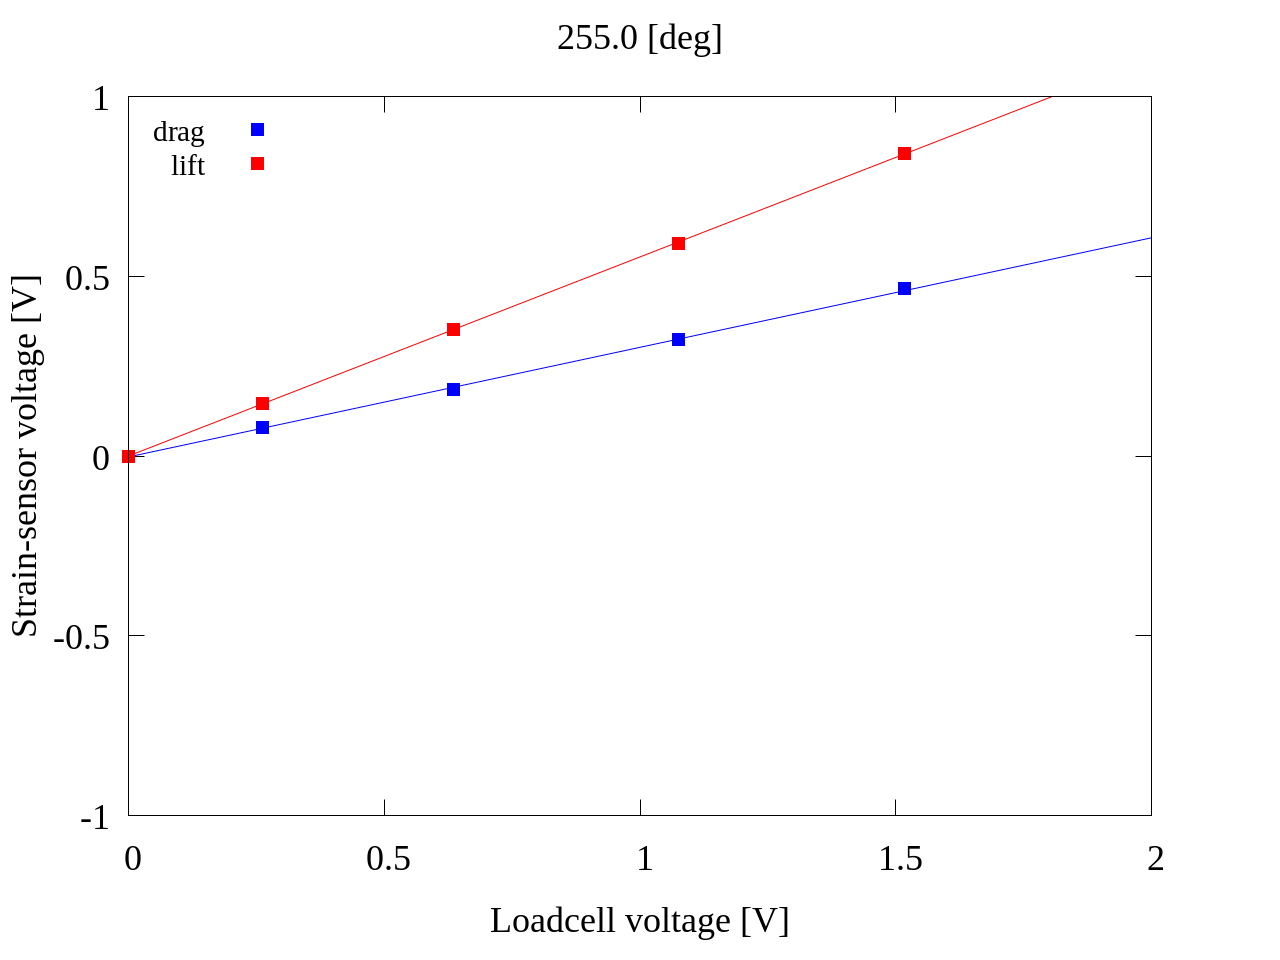
\includegraphics[width=70mm]{../../02_workspace/result/2-1/plot/04/04_linear_2550.png}
            \caption{Gradient of output voltage : 255 [deg]}
            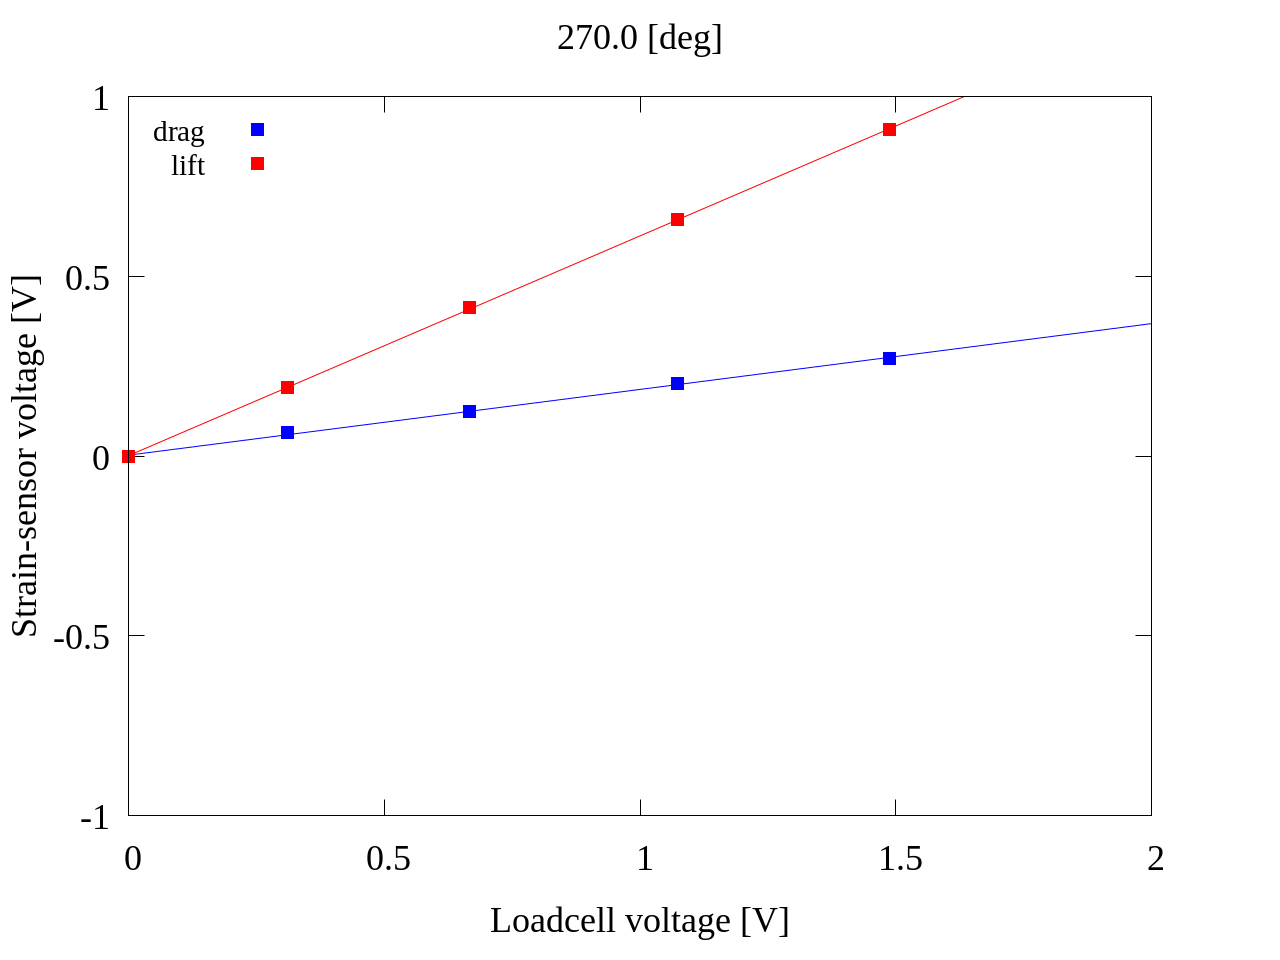
\includegraphics[width=70mm]{../../02_workspace/result/2-1/plot/04/04_linear_2700.png}
            \caption{Gradient of output voltage : 270 [deg]}
            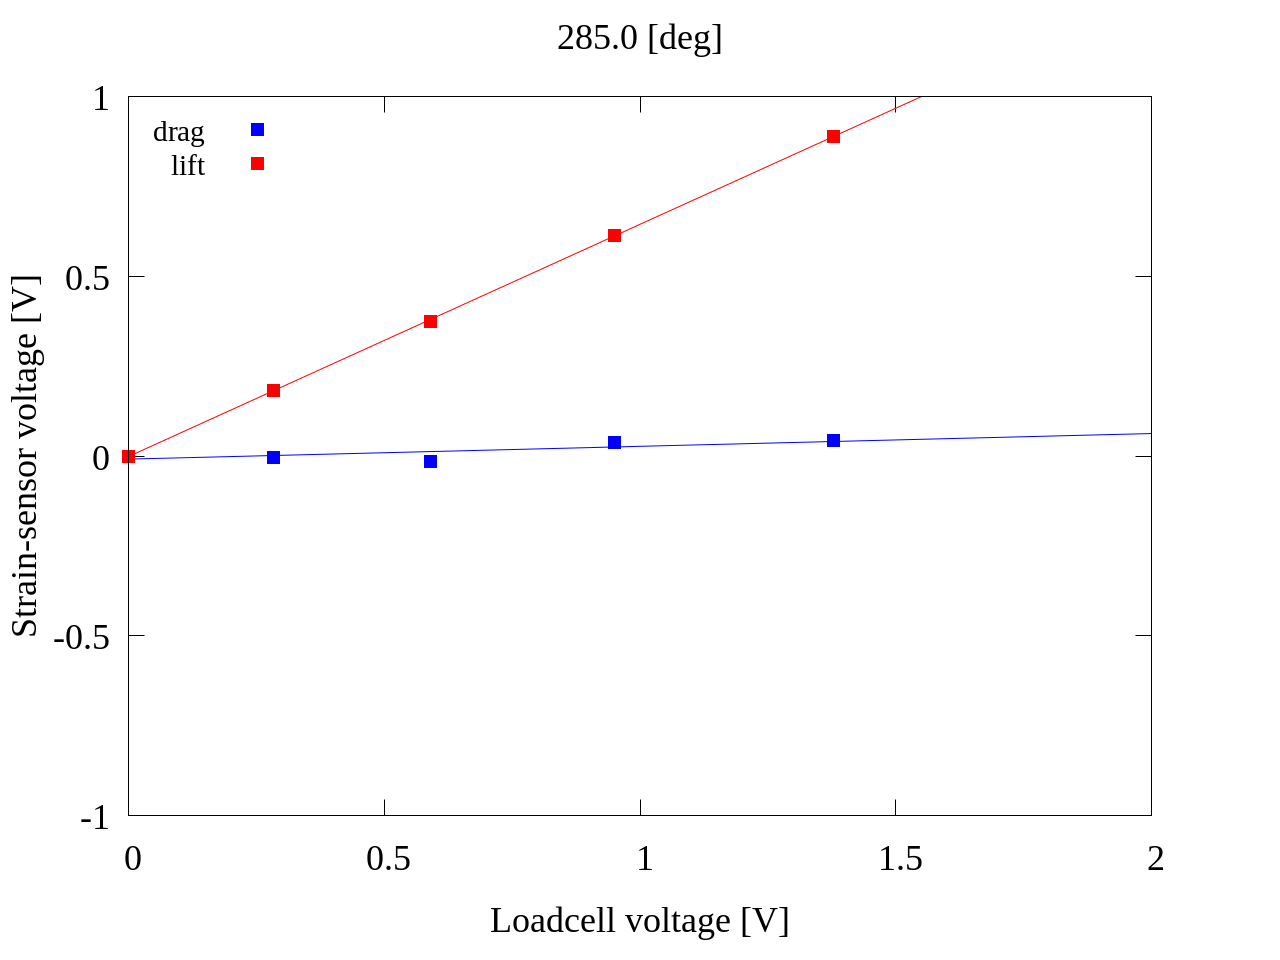
\includegraphics[width=70mm]{../../02_workspace/result/2-1/plot/04/04_linear_2850.png}
            \caption{Gradient of output voltage : 285 [deg]}
            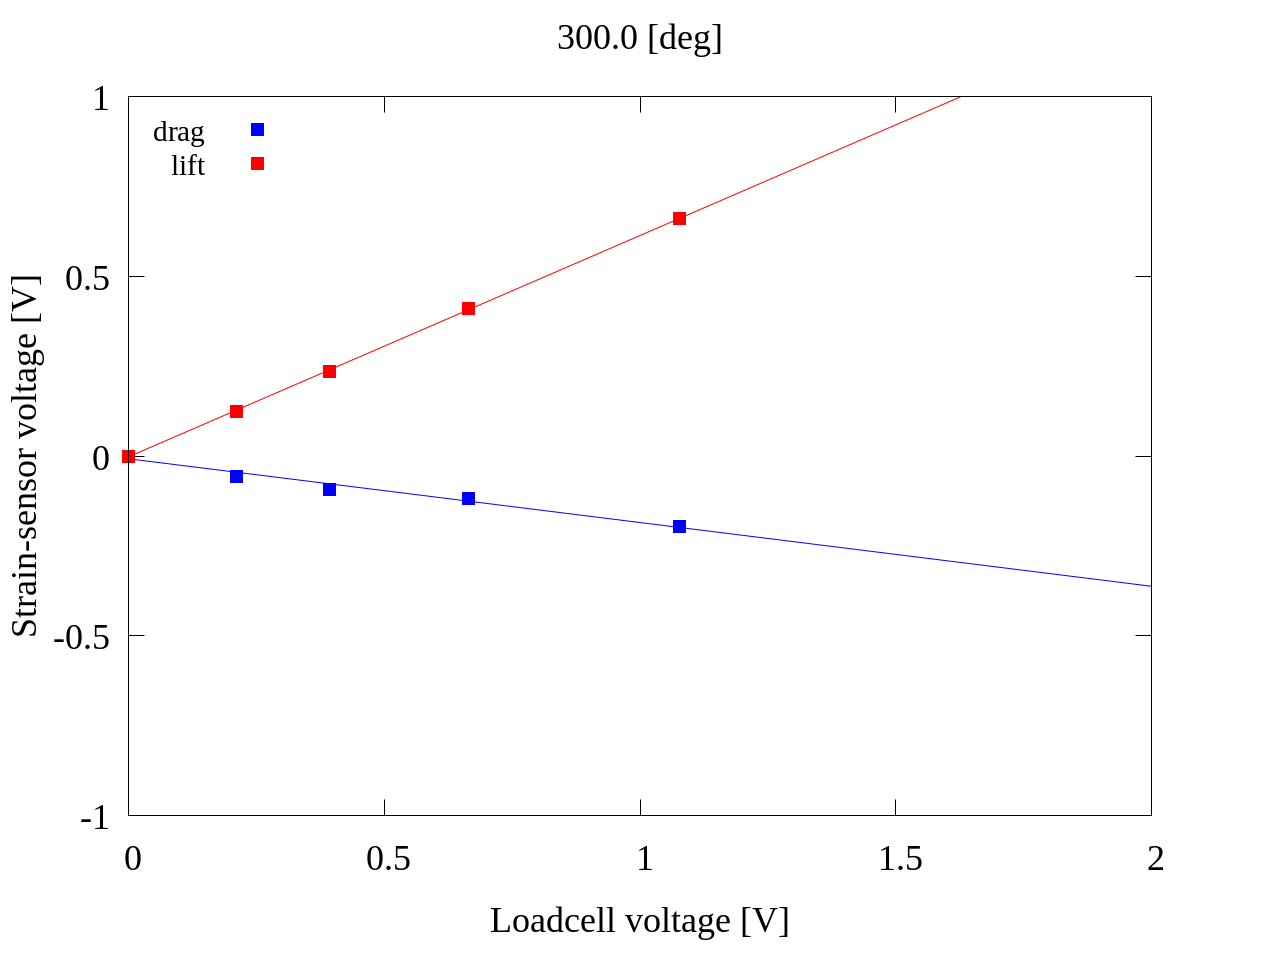
\includegraphics[width=70mm]{../../02_workspace/result/2-1/plot/04/04_linear_3000.png}
            \caption{Gradient of output voltage : 300 [deg]}
            \includegraphics[width=70mm]{../../02_workspace/result/2-1/plot/04/04_linear_3150.png}
            \caption{Gradient of output voltage : 315 [deg]}
            \includegraphics[width=70mm]{../../02_workspace/result/2-1/plot/04/04_linear_3300.png}
            \caption{Gradient of output voltage : 330 [deg]}
            \includegraphics[width=70mm]{../../02_workspace/result/2-1/plot/04/04_linear_3450.png}
            \caption{Gradient of output voltage : 345 [deg]}
        \end{center}
    \end{figure_here}
\end{multicols}

\newpage

また,以下のTable に,実験結果の出力電圧勾配の値を示す.

% \begin{table}[htbp]
%     \begin{center}
%         \caption{}
%         \begin{tabular}{|p{20mm}|p{20mm}|p{20mm}|}
%             \hline
%             \multicolumn{1}{|c|}{\textgt{Angle [deg]}} & \multicolumn{1}{|c|}{\textgt{$v_{d}}$ [V/V]}} & \multicolumn{1}{|c|}{\textgt{$v_{l}$ [V/V]}} \\ \hline
%             \multicolumn{1}{|c|}{0}                    & \multicolumn{1}{|r|}{}                        & \multicolumn{1}{|r|}{}                       \\ \hline
%             \multicolumn{1}{|c|}{15}                   & \multicolumn{1}{|r|}{}                        & \multicolumn{1}{|r|}{}                       \\ \hline
%             \multicolumn{1}{|c|}{30}                   & \multicolumn{1}{|r|}{}                        & \multicolumn{1}{|r|}{}                       \\ \hline
%             \multicolumn{1}{|c|}{45}                   & \multicolumn{1}{|r|}{}                        & \multicolumn{1}{|r|}{}                       \\ \hline
%             \multicolumn{1}{|c|}{60}                   & \multicolumn{1}{|r|}{}                        & \multicolumn{1}{|r|}{}                       \\ \hline
%             \multicolumn{1}{|c|}{75}                   & \multicolumn{1}{|r|}{}                        & \multicolumn{1}{|r|}{}                       \\ \hline
%             \multicolumn{1}{|c|}{90}                   & \multicolumn{1}{|r|}{}                        & \multicolumn{1}{|r|}{}                       \\ \hline
%             \multicolumn{1}{|c|}{105}                  & \multicolumn{1}{|r|}{}                        & \multicolumn{1}{|r|}{}                       \\ \hline
%             \multicolumn{1}{|c|}{120}                  & \multicolumn{1}{|r|}{}                        & \multicolumn{1}{|r|}{}                       \\ \hline
%             \multicolumn{1}{|c|}{135}                  & \multicolumn{1}{|r|}{}                        & \multicolumn{1}{|r|}{}                       \\ \hline
%             \multicolumn{1}{|c|}{150}                  & \multicolumn{1}{|r|}{}                        & \multicolumn{1}{|r|}{}                       \\ \hline
%             \multicolumn{1}{|c|}{165}                  & \multicolumn{1}{|r|}{}                        & \multicolumn{1}{|r|}{}                       \\ \hline
%             \multicolumn{1}{|c|}{180}                  & \multicolumn{1}{|r|}{}                        & \multicolumn{1}{|r|}{}                       \\ \hline
%             \multicolumn{1}{|c|}{195}                  & \multicolumn{1}{|r|}{}                        & \multicolumn{1}{|r|}{}                       \\ \hline
%             \multicolumn{1}{|c|}{210}                  & \multicolumn{1}{|r|}{}                        & \multicolumn{1}{|r|}{}                       \\ \hline
%             \multicolumn{1}{|c|}{225}                  & \multicolumn{1}{|r|}{}                        & \multicolumn{1}{|r|}{}                       \\ \hline
%             \multicolumn{1}{|c|}{240}                  & \multicolumn{1}{|r|}{}                        & \multicolumn{1}{|r|}{}                       \\ \hline
%             \multicolumn{1}{|c|}{255}                  & \multicolumn{1}{|r|}{}                        & \multicolumn{1}{|r|}{}                       \\ \hline
%             \multicolumn{1}{|c|}{270}                  & \multicolumn{1}{|r|}{}                        & \multicolumn{1}{|r|}{}                       \\ \hline
%             \multicolumn{1}{|c|}{285}                  & \multicolumn{1}{|r|}{}                        & \multicolumn{1}{|r|}{}                       \\ \hline
%             \multicolumn{1}{|c|}{300}                  & \multicolumn{1}{|r|}{}                        & \multicolumn{1}{|r|}{}                       \\ \hline
%             \multicolumn{1}{|c|}{315}                  & \multicolumn{1}{|r|}{}                        & \multicolumn{1}{|r|}{}                       \\ \hline
%             \multicolumn{1}{|c|}{330}                  & \multicolumn{1}{|r|}{}                        & \multicolumn{1}{|r|}{}                       \\ \hline
%             \multicolumn{1}{|c|}{345}                  & \multicolumn{1}{|r|}{}                        & \multicolumn{1}{|r|}{}                       \\ \hline
%         \end{tabular}
%     \end{center}
% \end{table}


\section{校正理論の適用とその結果}




\subsection{考察}